\chapter{Robust Compressive Sensing}
\index{Robust Compressive Sensing@\emph{Robust Compressive Sensing}}
\label{chp:robust-cs}

In this chapter, we develop LENS decomposition, a novel technique to accurately decompose network data represented in the form of a matrix into a low-rank matrix, a sparse anomaly matrix, an error term, and a small noise matrix. This decomposition naturally reflects the inherent structures of real-world data and is more general than existing compressive sensing techniques by removing the low-rank assumption and explicitly supporting anomalies.


\section{Analysis of Network Matrices}
\label{sec:measurement}

\begin{table}[htb]
  \centering
  {\small
    \vspace{-0.1in}
  \begin{tabular}{|@{~}l@{~~}|@{~~}l@{~}|@{~~}l@{~}|@{~~}l@{~}|@{~~}l@{~}|}
\hline
Network & Date & Duration & Resolution & Size  \\\hline
3G traffic & Nov. 2010 & 1 day & 10 min. & $472 \times 144$ \\\hline
WiFi traffic & Jan. 2013 & 1 day & 10 min. & $50 \times 118$ \\\hline
Abilene traffic~\cite{abilene} & Apr. 2003 & 1 week & 10 min. & $121 \times 1008$ \\\hline
G\'{E}ANT traffic~\cite{uhlig06:_provid} &  Apr. 2005 & 1 week  & 15 min. & $529 \times 672$ \\\hline
1 channel CSI & Feb. 2009 & 15 min. & 1 frame & $90 \times 9000$ \\\hline
multi. channels CSI & Feb. 2014 & 15 min. & 1 frame & $270 \times 5000$\\\hline  % 30 subcarriers * 9 channels
% Sensor & Feb. 2004 & 1 day & 10 min. & $54 \times 144$ \\\hline
Cister RSSI~\cite{RSSI1} & Nov. 2010 & 4 hours & 1 frame & $16 \times 10000$ \\\hline
CU RSSI~\cite{RSSI2} & Aug. 2007 & 500 frames & 1 frame & $895 \times 500$ \\\hline
UMich RSS~\cite{UMich-RSS} & April 2006 & 30 min. & 1 frame & $182 \times 3127$
\\\hline     % 14 * 13 pairs
UCSB Meshnet~\cite{UCSB-Meshnet} & April. 2006 & 3 days & 1 min. & $425 \times 1527$ \\\hline  % 38 * 38 pairs
%RON delay~\cite{RON} & Mar. 2001 & 2 days & 5 min. & $144 \times 494$ \\\hline
  \end{tabular}
  }
  \caption{Datasets under study.}
  \label{tab:data}
\end{table}

\subsection{Datasets}
\label{ssec:data}

Table~\ref{tab:data} lists the network matrices used for our
study. 
We obtained 3G traces from 472 base stations in a downtown area of a major city
% with a population of 8.7 million people,
in China during Oct. 2010. 
We generate traffic matrices by computing the aggregated traffic every 10
minutes. $M(i,t)$ represents the total traffic volume to and from base station
$i$ during time interval $t$, where $t$ is a 10-minute interval.
% A row in the traffic matrix represents the traffic time-series a base
% station while a column represents the aggregated traffic of base
% stations in the 10 minutes bin.

We also got WiFi traffic from a large university in China, and
generated traffic matrices based on the traffic collected at the 50 most
loaded access points (APs) on Jan. 4, 2013. $M(i, t)$ denotes
the total traffic to/from AP $i$ during the $t$-th 10-minute
time interval. 

In addition to wireless traffic matrices, we also
use traffic matrices from Abilene (Internet2)~\cite{abilene}
and G\'{E}ANT~\cite{uhlig06:_provid}, which are standard traffic matrices
used in several previous studies (\eg,
\cite{PCA2,lakhina04:_pca,anomography,zhang09sensing}) and useful for
comparison. Abilene traces report total end-to-end traffic between all pairs
in a 11-node network every 10 minutes. G\'{E}ANT traces report total traffic
between all pairs in a 23-node network every 15 minutes. 

For diversity, in addition to traffic matrices, we also obtain signal
strength and expected transmission time (ETT). % and Internet delay traces
We use the following SNR and RSS
matrices: (a) our 1 channel CSI traces, (b) our multi-channel CSI traces, (c) Cister RSSI traces, (d) CU
RSSI traces, and (e) UMich RSS. We collected (a) 
by having a moving desktop transmit back-to-back to another desktop and letting the receiving
desktop record the SNR across all OFDM subcarriers over 15 minutes
% sensor traces, and human traffic matrices in a social network.
% We get CSI traces by
% having two desktops as the sender and the receiver.
% Each desktop is
% equipped with
using the Intel Wi-Fi Link 5300 (iwl5300) adapter. The
modified driver~\cite{iwlagn} reports the channel matrices for 30
subcarrier groups in a 20MHz channel, which is about one group for every two subcarriers according to the standard~\cite{802.11n-2009}. The
sender sends 1000-byte frames using MCS 0 at a transmission power of
15 dBm. Since MCS0 has 1 stream and the receiver has 3 antennas, the
NIC reports CSI as a $90 \times 1$ matrix for each frame. 
% We walked
% with the sender and had the receiver record the CSI of the received
% frames for 15 minutes.
% The CSI matrix $M(t,f)$ denotes the SNR in the OFDM subcarrier group
% $f$ at time $t$. % An 802.11n channel consists of 30 OFDM
% subcarriers and the adapter has 3 antennas.
We collect (b) on channels 36, 40, 44, 48, 149, 153, 157, 161, and 165 at
 5GHz. The transmitter starts from channel 36, and sends 10 packets before
 switching to the next channel. The receiver synchronizes with the
 transmitter and also cycle through the 9 channels, which yields $270
 \times 1$ matrix for each frame.
In addition, we use Cister RSSI traces~\cite{RSSI1}, CU RSSI
traces~\cite{RSSI2}, and UMich RSS traces~\cite{UMich-RSS}, all of
which are publicly
available at CRAWDAD~\cite{crawdad}. $M(f,i)$ in Cister traces denotes
RSSI on IEEE 802.15.4 channel $f$ in the $i$-th frame,
$M(l,i)$ in CU traces denotes RSSI of the $i$-th frame at location
$l$, and $M(s,i)$ in UMich-RSS trace denotes the RSS measurement 
received by the $s$-th sensor pair in the $i$-th packet.
% We get sensor traces from Intel Berkeley Research Lab where they collected  temperature, humidity, light, and voltage information from 54 sensor nodes between February 28, 2004 and April 5, 2004~\cite{intel_sensor}. %We generate human traffic matrices by ...
We also use ETT traces from UCSB Meshnet~\cite{UCSB-Meshnet}, % and
% resilient overlay trace~\cite{RON}. 
% UCSB Meshnet~\cite{UCSB-Meshnet}
which contains the ETT of every links in a 20-node mesh network. 
We generate the ETT matrix $M(l,t)$, where $M(l,t)$ denotes the ETT of
the link $l$ during the $t$-th 10-second window.
% RON trace contains end-to-end delay of packets sent
% between any pairs of nodes in a 12-node overlay network. We generate
% delay matrix $M(i,t)$, where $M(i,t)$ denotes the average delay
% between the $i$-th node pair during the $t$-th 5-minute time interval.

\begin{figure}[h!]
  \centering
  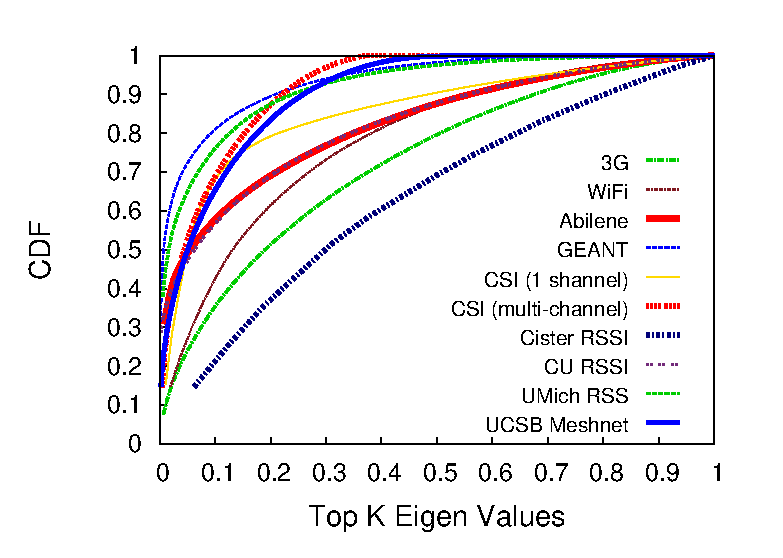
\includegraphics[width=\figurewidthA]{fig/matrix.na0.anom0.rank.eps}
  % \caption{CDF of energy that are contained in the top K singular values
  %   of the original matrices.}
  \caption{CDF of ranks.}
  \label{fig:original-matrix-rank}
\end{figure}

\subsection{Analysis}
\label{ssec:analysis}

\para{Rank analysis:} For each network matrix, we mean center each row (\ie, subtract from
each row its mean value).  We then apply singular value decomposition
(SVD) to examine if the mean-centered matrix has a good low-rank
approximation.  The metric we use is the fraction of total variance
captured by the top $K$ singular values, \ie, $\left({\sum_{i=1}^{K}
  s_i^2}\right)/\left({\sum_{i} s_i^2}\right)$, where $s_i$ is the
$i$-th largest singular value and $\left({\sum_{i} s_i^2}\right)$
gives the total variance of the mean-centered coordinate matrix.  Note
that $1 - \left({\sum_{i=1}^{K} s_i^2}\right)/\left({\sum_{i}
  s_i^2}\right)$ is the relative approximation error of the best
rank-$K$ approximation with respect to the squared Frobenius norm.

Figure~\ref{fig:original-matrix-rank} plots the fraction of total
variance captured by the top $K$ singular values for different
traces. 
As it shows,
% some matrices are low rank. For example, 
% G\'{E}ANT takes 20.8\% singular values to capture 90\%
% variance in the original matrices. 
% However, there are also some matrices are not low rank. 3G 
% and Cister RSSI matrices take 68.1\% and 81.0\% singular values to
% capture 90\% variance respectively.
% We further inject anomalies to see how it affects the results. 
% These results show XXX
from low to high, UCSB Meshnet, G\'{E}ANT, multi-channel CSI, UMich RSS, RON, 
1-channel CSI, CU RSSI, Abilene, WiFi, 3G, and Cister RSSI
matrices take 7.5\%, 20.8\%, 22.0\%, 23.9\%, 47.2\%, 
48.9\%, 55.8\%, 57.0\%, 58.0\%, 68.1\%, and 81.0\%
singular values to capture 90\% variance, respectively. Therefore,
only UCSB Meshnet, G\'{E}ANT, multi-channel CSI, and UMich RSS are
close to low rank.

\begin{figure}[h!]
  \centering
  \subfigure[\small{5\% anomalies with s=0.5}]{
    \includegraphics[width=\figurewidthB]{fig/matrix.na0.05.anom0.5.rank.eps}
  }
  \subfigure[\small{10\% anomalies with s=0.5}]{
    \includegraphics[width=\figurewidthB]{fig/matrix.na0.1.anom0.5.rank.eps}
  }
  \subfigure[\small{5\% anomalies with s=1}]{
    \includegraphics[width=\figurewidthB]{fig/matrix.na0.05.anom1.rank.eps}
  }
  \subfigure[\small{10\% anomalies with s=1}]{
    \includegraphics[width=\figurewidthB]{fig/matrix.na0.1.anom1.rank.eps}
  }
  \caption{Ranks under anomalies in traffic matrices.}
  \label{fig:anomalous-traffic-matrix-rank}
\end{figure}

%[also update numbers. Pick a couple of wireless traces instead of
%  Geant to focus on.]  
Next we inject anomalies to see how it affects
the results.  We inject anomalies to a portion of the entries in the
original matrices. Following the standard anomaly injection method
used in existing work~\cite{PCA2, decentralized_PCA, P3CA}, 
we first use exponential weighted
moving average (EWMA) to predict the future entries based on their
past values (\ie, $y=\alpha x + (1-\alpha)y$, where $\alpha=0.8$ in
our evaluation) and use the maximum difference between the actual and
predicted value as the anomaly size to be injected. We vary the
fraction of entries to inject anomalies from 5\% to 10\%, and also
scale the anomaly size by $s$, which is 0.5 or 1. As shown in
Figure~\ref{fig:anomalous-traffic-matrix-rank}, 
% For Abilene, G\'{E}ANT, 3G, and WiFi traffic matrices and RON delay
% matrices, we first normalize each matrix by dividing each entry by the
% maximum element in the matrix. We then inject anomalies by adding or
% subtracting (with equal probability) a number randomly drawn from a
% uniform distribution between $(s,2s)$. We then ensure all entries are
% no smaller than 0 after injecting anomalies, since traffic and delay
% matrices take non-negative values. We vary $s$ and the number of
% entries to which anomalies are injected.
% For convenience, we call $x$ as anomaly size.
when we inject more anomalies or larger anomalies, more singular values are
required in order to capture the variance of the matrices. This trend
is consistent across all traces. For example, as shown in
Figure~\ref{fig:anomalous-traffic-matrix-rank}(a)-(b), 
when we inject 5\% and 10\% anomalies with s=0.5, it takes 60.9\% and
67.6\% singular values to capture 90\% variance in UMich Meshnet, 
71.0\% and 75.8\% in WiFi trace, and 75.7\% and 80.0\% in 1-channel CSI trace.
As shown in
Figure~\ref{fig:anomalous-traffic-matrix-rank}(c)-(d), 
when we inject 5\% and 10\% anomalies with s=1, the corresponding numbers
are 72.5\% and 76.9\% in UMich Meshnet, 72.0\% and 78.3\% in WiFi trace,
and 81.7\% and 84.1\% in 1-channel CSI trace.
% Similarly, but not shown for
% brevity, it takes 79.3\% and 81.8\% singular values for Abilene to
% capture 90\% variance, when we inject 5\% and 10\% anomalies with an
% average size of 0.1, respectively.  The corresponding numbers rose to
% 85.1\% and 86.0\% when we inject 5\% and 10\% anomalies with an
% average size of 0.5, respectively.
The other matrices exhibit the same trend.

% \begin{figure}[h!]
%   \centering
%   \hspace{-0.2in}
%   \subfigure[\small{5\% anomalies with k=1}]{
%     \includegraphics[width=1.0\figurewidthA]{fig/matrix.na0.05.anom2.rank.eps}
%   }
%   \hspace{-0.2in}
%   \subfigure[\small{10\% anomalies with k=1}]{
%     \includegraphics[width=1.0\figurewidthA]{fig/matrix.na0.1.anom2.rank.eps}
%   }
%   \hspace{-0.2in}
%   \subfigure[\small{5\% anomalies with k=2}]{
%     \includegraphics[width=0.99\figurewidthA]{fig/matrix.na0.05.anom4.rank.eps}
%   }
%   \hspace{-0.2in}
%   \subfigure[\small{10\% anomalies with k=2}]{
%     \includegraphics[width=0.99\figurewidthA]{fig/matrix.na0.1.anom4.rank.eps}
%   }
%   \vspace{-0.1in}
%   \caption{CDF of energy that are contained in the top K singular values
%     under anomalies in CSI and RSSI traces.}
%   \vspace{-0.1in}
%   \label{fig:anomalous-rssi-matrix-rank}
% \end{figure}

% We also inject anomalies to SNR and RSS traces. Since the elements in
% SNR and RSS traces have dB as a unit, we use a different way of
% injecting anomalies. We inject anomalies by adding or subtracting a
% number randomly drawn from a uniform distribution between $(k*std,
% 2k*std)$, where $std$ is standard deviation of all elements in a
% matrix. Figure~\ref{fig:anomalous-rssi-matrix-rank} shows the results
% for k=1 and 2. Again we observe the same trend -- the presence of more
% anomalies and larger anomalies increases the rank of the matrix.

\begin{figure}[h!]
  \centering
  \includegraphics[width=1\columnwidth]{fig/legend_temporal.eps}
  \subfigure[\small{k=1}]{
    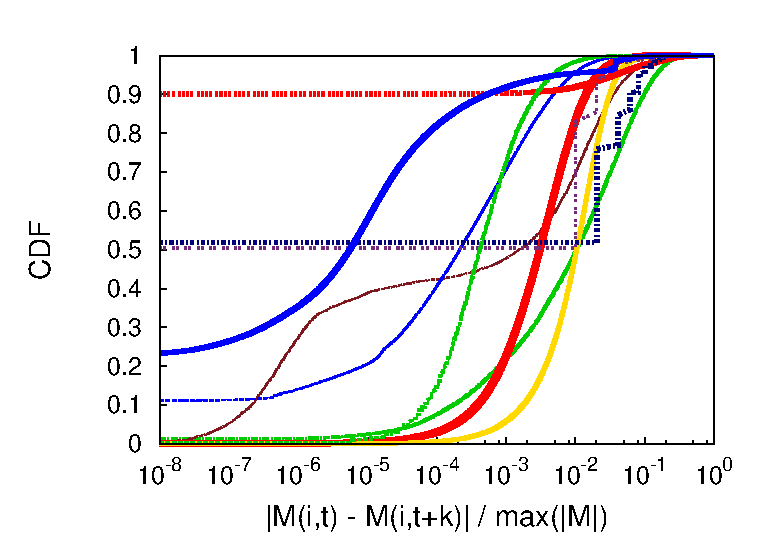
\includegraphics[width=\figurewidthB]{fig/matrix.na0.anom0.itvl1.diff.eps}
  }
  \subfigure[\small{k=10}]{
    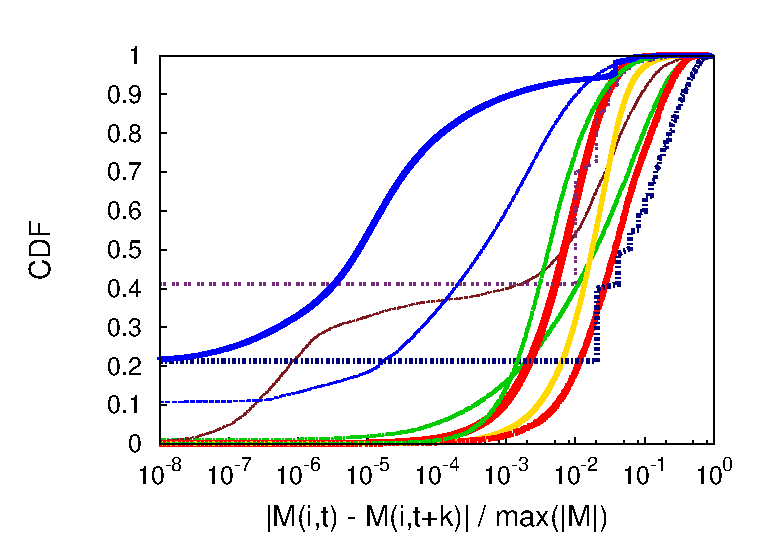
\includegraphics[width=\figurewidthB]{fig/matrix.na0.anom0.itvl10.diff.eps}
  }
  % \caption{CDF of normalized difference between i-th and i+k-th time slot.}
  \caption{CDF of normalized difference between time slots.}
  \label{fig:temporal-stability}
\end{figure}


\para{Temporal stability:} Figure~\ref{fig:temporal-stability} plots the CDF of
normalized temporal variation (\ie, $\frac{x(i)-x(i-t)}{max(x(i))}$)
across different traces. As it shows, different traces exhibit
varying degrees of temporal stability. For example, 3G and Cister RSSI have
high variation: the two adjacent entries differ by 6.1\%-9.8\% in 90\%
cases, and 10 time-slot apart entries differ by 16.7\%-36.2\% in 90\%. 
In comparison, UMich Meshnet and G\'{E}ANT have low variation, where the adjacent
entries differ by 0.3\%-0.5\% in 90\% cases and 10 time-slot apart
entries differ by 1.0\%-2.4\% in 90\%. The other traces are in between.

\para{Summary:} The major findings from the above analysis include: (i) Not
all real network matrices are low rank. (ii) Adding anomalies further
increases the rank. (iii) Temporal stability varies substantially
across different traces. These findings motivate us to develop a
general compressive sensing framework to support diverse matrices that
may not be low rank, exhibit different degrees of temporal stability,
and may even contain anomalies.


%% =================================================================

\section{LENS Decomposition}
\label{sec:lens}

In this section, we first present LENS decomposition framework. Next we develop
an alternating direction method for solving the decomposition
problem. Then we describe how to set the parameters.

\subsection{LENS Decomposition Framework}
\label{ssec:lens}

\para{Overview:} There are many factors that contribute to
real network matrices, including measurement errors, anomalies and
inherent noise.  To capture this insight, we decompose the
original matrix into a {\underline L}ow-rank component, an
{\underline E}rror component, a {\underline N}oise component, and a
{\underline S}parse anomaly component (hence the acronym
{\underline{LENS}} decomposition). This is motivated by the following
observations:
\begin{sitemize}
\item Low-rank component: Network matrices often exhibit significant redundancy.
A concrete form of redundancy is that the network matrix of interest
can be well approximated by low-rank matrices.  For example, TM
estimation makes use of the gravity model~\cite{ZRDG03}, which is
essentially a rank-1
approximation to matrices. \cite{mobile-localization}
uses low-rank matrices for localization.
\item Sparse component: Anomalies are common in large network dataset.
  Anomalies may arise from a number of factors. For example,
  traffic anomalies may be caused by problems ranging from security
  threats (\eg, Distributed Denial of Service (DDoS) attacks and
  network worms) to unusual traffic events (\eg, flash crowds), to
  vendor implementation bugs, and to network misconfigurations.  Such
  anomalies are typically not known a priori and are sparse~\cite{anomaly_sparsity, anomaly_sparsity2}.


Note that there can be systematic effects that are only
sparse after some transformation (\eg, wavelet transform).  For
example, a major level shift may result in persistent changes in the
original data (and is thus not sparse).  But after wavelet transform
(or simple temporal differencing), it becomes sparse. 

\item Error and artifacts: The measurement and data collection procedure
may also introduce artifacts. For example, a SNMP traffic counter may wrap
around, resulting in negative measurements.
One can always try his best to apply domain knowledge to filter out
obvious errors and artifacts (\eg, missing data or negative traffic
measurements).  However, in general it is difficult to filter out all
such artifacts.  The advantage of considering both anomalies and
errors jointly is that the parts that cannot be filtered can get
absorbed by the sparse components.

\item Noise.  Noise is universal, making clean mathematical models
approximate in practice. For example, real-world network matrices are
typically only approximately low-rank as opposed to exactly low-rank.

%\item Locality. Network data may also exhibit spatial or temporal
%locality \cite{anomaly_spatio_temporal,Wang:2002:model_spatio_temporal,
% George:2007:spatio_temporal_database}. 
% For example, traffic 
% at similar point of time may be similar. 
% Temperature at similar locations are similar.
\end{sitemize}


% Considering all these effects.
Therefore a natural approach is to consider the
original dataset as a mixture of all these effects.  It is useful if
one can decompose the original matrix into individual components, each
component capturing one major effect.

\para{Basic formulation:} The basic LENS decomposition decomposes an original $m\times n$ data matrix $D$ into
a low-rank matrix $X$, a sparse anomaly matrix $Y$, a noise matrix
$Z$, and an error matrix $W$.  This is achieved by solving the
following {\em convex} optimization problem:
\begin{eqnarray}
\text{minimize:} && \alpha \|X\|_* + \beta \|Y\|_1 + 
                    \frac{1}{2\sigma}\|Z\|_F^2, \nonumber\\
\text{subject to:}&& X + Y + Z + W = D, \nonumber\\
&& E.*W = W.
\label{eq:lens-basic}
\end{eqnarray}
where $X$ is a low-rank component, $Y$ is a sparse anomaly component,
$Z$ is a dense noise term, and $E$ is a binary error indicator matrix
such that $E[i,j] = 1$ if and only if entry $D[i,j]$ is erroneous or
missing, and $W$ is an arbitrary error component with $W[i,j] \neq 0$
only when $E[i,j] = 1$ (thus $E.*W = W$, where $.*$ is an element-wise
multiplication operator). Since $W$ fully captures the erroneous or
missing values, we can set $D[i,j] = 0$ whenever $E[i,j] = 1$ without
loss of generality. The constraint enforces $D$ to be the sum of $X$,
$Y$, and $Z$ when $D$ is neither missing nor has errors (since
$E[i,j].*W[i,j] = 0$ in this case), while imposing no constraint when
$D$ is missing or has error (since $E[i,j].*W[i,j]=W[i,j]$ allows
$W[i,j]$ to take an arbitrary value to satisfy $X+Y+Z+W=D$).

The optimization objective has the following three components:
\squishlist
\item $\|X\|_*$ is the nuclear norm~\cite{recht08:_nec,recht:_guaran} of
  matrix $X$, which penalizes against high rank of $X$ and can be
  computed as the total sum of $X$'s singular values.

\item $\|Y\|_1$ is the $\ell_1$-norm of $Y$, which penalizes against
  lack of sparsity in $Y$ and can be computed as $\|Y\|_1 = \sum_{i,j}
  |Y[i,j]|$.

\item $\|Z\|_F^2$ is the squared Frobenius norm of matrix $Z$, which
penalizes against large entries in the noise matrix $Z$ and can be computed as
$\|Z\|_F^2 = \sum_{i,j} Z[i,j]^2$.

\squishend

The weights $\alpha$, $\beta$ and $\frac{1}{2\sigma}$ balance the
conflicting goals to simultaneously minimize $\|X\|_*$, $\|Y\|_1$ and
$\|Z\|_F^2$.  We describe how to choose these weights in
Section~\ref{ssec:para}.  


\para{Generalized formulation:} Below we generalize both the
constraints and the optimization objective of the basic formulation in
Eq.~\eqref{eq:lens-basic} to accommodate rich requirements in the
analysis of real-world network matrices.

%\begin{sitemize}
  
%\item
First, the matrix of interest may not always be directly observable,
  but its linear transform can be observed though subject to missing
  data, measurement errors, and anomalies. For example, end-to-end
  traffic matrices $X$ are often not directly observed, and what can
  be observed are link load $D$. $X$ and $D$ follow $AX = D$, where
  $A$ is a binary routing matrix: $A(i,j) =
  1$ if link $i$ is used to route traffic for the $j$-th end-to-end
  flow, and $A(i,j) = 0$ otherwise.  We generalize the constraints in
  Eq.~\eqref{eq:lens-basic} to cope with such measurement
  requirements:
\begin{equation}
 AX + BY + CZ + W = D
\end{equation}
Here $A$ may capture tomographic constraints that linearly relate
direct and indirect measurements (\eg, 
$A$ is a routing matrix in the traffic matrices).  $B$ may represent an over-complete anomaly
profile matrix. If we do not know which matrix entries may have
anomalies, we can simply set $B$ to the identity matrix $I$. It is also
possible to set $B=A$ if we are interested in capturing anomalies in
$X$.  Without prior knowledge, we set $C$ to be the identity
matrix.



Prior research on network inference and compressive sensing
  highlights the importance of incorporating domain knowledge about
  the structure of the underlying data. To capture domain knowledge,
  we introduce one or more penalty terms into the
  optimization objective: $\sum_{k=1}^K \|P_k X Q_k^T - R_k\|_F^2$,
  where $K$ is the number of penalty terms.  We also introduce a
  weight $\gamma$ to capture our confidence in such knowledge.

Examples of domain knowledge include temporal stability constraints,
spatial locality constraints, and initial estimation of $X$ (\eg,
\cite{ZRDG03} derives initial traffic matrices using the gravity
model~\cite{gravity1}). Temporal and spatial locality are common 
in network data~\cite{anomaly_spatio_temporal,Wang:2002:model_spatio_temporal,George:2007:spatio_temporal_database}. Such domain knowledge is especially helpfulwhen there are many missing entries, making the problem severely
under-constrained.
%locality . 
% For example, traffic 
% at similar point of time may be similar. 
% Temperature at similar locations are similar.

Consider a few simple cases. First, when
$k=1$, $P_1$ is an identity matrix $I$, $R_1$ is a zero vector, we can
set $Q_1=Toeplitz(0,1,-1)$, which denotes the Toeplitz matrix with
central diagonal given by ones, the first upper diagonal given by
negative one, \ie,
\begin{equation}
  Q = \left[
   \begin{array}{rrrrrrrr}
         1 & -1 &  0 &  0 &  \ldots \\
         0 &  1 & -1 &  0 & \ddots \\
         0 &  0 &  1 & -1 & \ddots \\
         \vdots &  \ddots &  \ddots & \ddots &  \ddots   \\
   \end{array} \right].
\end{equation}
$Q^T$ denotes the transpose of matrix $Q$. $P_1 X Q_1^T$ captures the
differences between two temporally adjacent elements in
$X$. Minimizing $\|P_1 X Q_1^T - R_1\|_F^2=\|P_1 X Q_1^T\|_F^2$
reflects the goal of making $X$ temporally stable. For simplicity,
this is what we use for our evaluation. In general, one can use
similar constraints to capture other temporal locality patterns during
different periods (\eg, seasonal patterns or diurnal patterns).

Next we consider the spatial locality, which is represented by $P$. If
$k=1$, $R_1=0$, $Q_1$ is an identity matrix $I$, we can set $P_1$ to
reflect the spatial locality. For example, if two adjacent elements in
the matrix have similar values, we can set $P =
Toeplitz(0,1,-1)$. Similarly, if different parts of the matrix have
different spatial locality patterns, we can use different $P$'s to
capture these spatial locality patterns. For simplicity, our
evaluation considers only temporal stability, which is well known to
exist in different networks. We plan to incorporate spatial locality
in the future.

% We also selectively evaluate the spatial locality
% on some matrices that are likely to exhibit locality (\eg, CSI
% matrices where SNR on adjacent frequencies should be similar).

Finally, if we have good initial estimate of $X_{init}$ (\eg, \cite{ZRDG03}
uses the gravity model to derive the initial TM), we can
leverage this domain knowledge by minimizing $\|X - X_{init}\|$ (\ie, $R_1=X_{init}$). This
term can be further combined with spatial and/or temporal locality to
produce richer constraints.

%\end{sitemize}  

Putting everything together, the general formulation is:

{\small
\begin{eqnarray}
\text{minimize:}  && \alpha \|X\|_* + \beta \|Y\|_1 +
\frac{1}{2\sigma}\|Z\|_F^2 +\frac{\gamma}{2\sigma}\sum_{k=1}^K\|P_k X Q_k^T - R_k\|_F^2, \nonumber\\
\text{subject to:}&& AX + BY + CZ + W = D, \nonumber\\
&& E.*W = W.
\label{eq:general-lens-basic}
\end{eqnarray}
}
Note that our formulation is more general than recent research on
compressive sensing
(\eg,~\cite{zhang09sensing,robustPCA,recht08:_nec,recht:_guaran}),
which do not consider anomalies,
% (typically only 2 or 3 components out of $\{X,Y,Z,W\}$),
have simpler constraints (\eg, there is no
$A$, $B$, or $C$), and have less general objectives.

% XXX  For example, to
% enumerate all possible spike locations, we can simply set $B$ to be
% the identity matrix $I$.  % Alternatively, $B$ can also be constructed
% using Haar wavelet transform matrix, or the discrete cosine transform
% matrix, or a combination of these.
% We ensure that columns of $B$ are
% distinct and have unit length. % $C$ is XXX.

%In this case, we observe that (i) when $X$ is low-rank, $AX$ is also
%low-rank, and (ii) when $Z$ is a dense noise matrix, $CZ$ is also
%likely to be dense.  We therefore propose to infer $X$, $Y$, $Z$, and
%$W$ by solving
%\begin{eqnarray}
%\text{minimize:}  && \alpha \|AX\|_* + \beta \|Y\|_1 
%                    +\frac{1}{2\sigma}(\|T*Q^T\|_F^2+\|CZ\|_F^2), \nonumber\\
%\text{subject to:}&& AX + BY + T + CZ + E.*W = D, \label{eq:lens-general}
%\end{eqnarray}  
%where $\sigma$ becomes the standard deviation of (non-erroneous)
%elements of $CZ$ instead of $Z$.

\subsection{Optimization Algorithm}
\label{ssec:adm}

The generality of the formulation in Eq.~\eqref{eq:general-lens-basic}
makes it challenging to optimize. We are not aware of any
existing work on compressive sensing that can cope with such a general
formulation.  Below we first reformulate
Eq.~\eqref{eq:general-lens-basic} to make it easier to solve.  We then
consider the augmented Lagrangian function of the reformulated problem
and develop an Alternating Direction Method to solve it.

\para{Reformulation for optimization:} Note that $X$ and $Y$ appear in
multiple locations in the objective function and constraints in the
optimization problem~\ref{eq:general-lens-basic}. This coupling makes
optimization difficult. To reduce coupling, we introduce a set of
auxiliary variables $X_0,X_1,\cdots,X_{K}$ and $Y_0$ and reformulate
the problem as follows:
\begin{eqnarray}
\text{minimize:}  && \alpha \|X\|_* + \beta \|Y\|_1 +
\frac{1}{2\sigma}\|Z\|_F^2 \nonumber\\
                  && \quad+\frac{\gamma}{2\sigma}\sum_{k=1}^K\|P_k X_k Q_k^T - R_k\|_F^2, \nonumber\\
\text{subject to:}&& AX_0 + BY_0 + CZ + W = D, \nonumber\\
&& E.*W = W, \nonumber\\
&& X_k - X = 0\quad (\forall k=0,\cdots,K\nonumber),\\
&& Y_0 - Y = 0.
\label{eq:reformulated-lens}
\end{eqnarray}
where $Y_0$ and $X_{k} (0\leq k \leq K)$ are auxiliary variables.
Note that formulations Eq.~\eqref{eq:reformulated-lens} and
Eq.~\eqref{eq:general-lens-basic} are equivalent.

\comment{ %old lens
Note that we can simplify Eq.~\eqref{eq:lens-general} by performing a
change of variable.  Specifically, let $X = A X_{\mathrm{orig}}$ and
$Z = C Z_{\mathrm{orig}}$, then Eq.~\eqref{eq:lens-general} becomes:
\begin{eqnarray}
\text{minimize:}  && \alpha \|X\|_* + \beta \|Y\|_1 +
                     \frac{1}{2\sigma}(\|T*Q^T\|_F^2 + \|Z\|_F^2), \nonumber\\
\text{subject to:}&& X + BY + T + Z + E.*W = D. \label{eq:lens-simple}
\end{eqnarray}  

Once we solve Eq.~\eqref{eq:lens-simple}, we can then infer
$X_{\mathrm{orig}}$ and $Z_{\mathrm{orig}}$ according to
$X_{\mathrm{orig}} = \mathsf{pinv}(A) X$ and $Z_{\mathrm{orig}} =
\mathsf{pinv}(C) Z$, where $\mathsf{pinv}(M)$ is the pseudo-inverse
of matrix $M$.  
}

\para{Alternating Direction Method for solving
  \eqref{eq:reformulated-lens}:} We apply an Alternating Direction
Method (ADM)~\cite{adm} to solve the convex optimization problem in
~\eqref{eq:reformulated-lens}.  Specifically, we consider the
augmented Lagrangian function:

\begin{small}
\begin{eqnarray}
\lefteqn{\mathcal{L}(X,\{X_k\},Y,Y_0,Z,W,M,\{M_k\},N,\mu)}\nonumber\\
\defas&&\alpha\|X\|_* + \beta\|Y\|_1 + \frac{1}{2\sigma}\|Z\|_F^2\nonumber\\
&&   +~ \frac{\gamma}{2\sigma} \sum_{k=1}^K \|P_k X_k Q_k^T-R_k\|_F^2\nonumber\\
&&   +~ \langle M,D-AX_0-BY_0-CZ-W \rangle \label{eq:lang1}\\ 
&&   +~ \sum_{k=0}^K\langle M_k,X_k-X\rangle \label{eq:lang2}\\
&&   +~ \langle N,Y_0-Y \rangle \label{eq:lang3}\\
&&   +~ \frac{\mu}{2}\cdot \|D-AX_0-BY_0-CZ-W\|_F^2 \label{eq:penalty1}\\
&&   +~ \frac{\mu}{2}\cdot \sum_{k=0}^K \|X_k-X\|_F^2 \label{eq:penalty2}\\
&&   +~ \frac{\mu}{2}\cdot \|Y_0-Y\|_F^2 \label{eq:penalty3}
\end{eqnarray}
\end{small}
where $M$, $\{M_k\}$, $N$ are the Lagrangian
multipliers~\cite{lag-multiplier} for the equality constraints in
Eq.~\eqref{eq:reformulated-lens}, and $\langle U, V\rangle \defas
\sum_{i,j} (U[i,j] \cdot V[i,j])$ for two matrices $U$ and $V$ (of the
same size).  Essentially, the augmented Lagrangian function includes
the original objective, three Lagrange multiplier terms
\eqref{eq:lang1}--\eqref{eq:lang3}, and three penalty terms converted
from the equality constraints
\eqref{eq:penalty1}--\eqref{eq:penalty3}.  Lagrange multipliers are
commonly used to convert an optimization problem with equality
constraints into an unconstrained one.  Specifically, for any optimal
solution that minimizes the (augmented) Lagrangian function, the
partial derivatives with respect to the Lagrange multipliers must be
0.  Hence the original equality constraints will be satisfied.  The
penalty terms enforce the constraints to be satisfied.  The benefit of
including Lagrange multiplier terms in addition to the penalty terms
is that $\mu$ no longer needs to iteratively increase to $\infty$ to
solve the original constrained problem, thereby avoiding
ill-conditioning~\cite{adm}.  Note that we do not include terms
corresponding to constraint $E.*W=W$ in the augmented Lagrangian
function, because it is straightforward to enforce this constraint
during each iteration of the Alternating Direction Method without the
need for introducing additional Lagrange multipliers.

%\begin{eqnarray*}
%&\mathcal{L}(X,Y,Z,W,T,M,\mu) \\
%\defas&\alpha\|X\|_* + \beta|Y|_1 +  \frac{1}{2\sigma} (\|Z\|_F^2 +\|T*Q^T\|_F^%2)  \\
%&+ \langle M, D-X-BY-Z-T-W \rangle \\
%&+ \frac{\mu}{2}\|D-X-BY-Z-T-W\|_F^2,
%\end{eqnarray*}
%where $M$ is the Lagrange multipliers for constraints
%$D-X-BY-Z-T-W=0$, and $\langle M, N\rangle = \sum_{i,j} (M[i,j] \cdot
%N[i,j]) = \mathsf{trace}(M\cdot N)$ is the trace of $M\cdot N$.

The ADM algorithm progresses in an iterative fashion.  During each
iteration, we alternate among the optimization of the augmented
Lagrangian function by varying each one of $X$, $\{X_k\}$, $Y$, $Y_0$,
$Z$, $W$, $M$, $\{M_k\}$, $N$ while fixing the other variables.  
Introducing auxiliary variables $\{X_k\}$ and $Y_0$ makes it
possible to obtain a close-form solution for each optimization
step. Following ADM, 
% The procedure is guaranteed to converge quickly if
we increase $\mu$ by a constant factor $\rho \geq 1$ during each
iteration.  When involving only two components, ADM is guaranteed to
converge quickly.  In our general formulation, convergence is no
longer guaranteed, though empirically we observe quick convergence in
all our experiments (\eg, as shown in Section~\ref{sec:eval}).  We
plan to apply techniques in \cite{convergence} to ensure guaranteed
convergence in future work. We further improve efficiency by
replacing exact optimization with approximate optimization during each
iteration. Appendix~\ref{appendix:adm} gives a detailed description on
the steps during each iteration.

\para{Improving efficiency through approximate SVD:} The most
time-consuming operation during each iteration of the Alternating
Direction Method is performing the singular value decomposition.  In
our implementation, we add an additional constraint on the rank of
matrix $X$: $ rank(X) \leq r$, where $r$ is a user-specified parameter
that represents an estimated upper bound on the true rank of $X$.  We
then explicitly maintain the SVD of $X$ and update it approximately
during each iteration through the help of rank-revealing QR
factorization of matrices that have only $r$ columns (which are much
smaller than the original matrices used in SVD).  We omit the details
of approximate SVD in the interest of space.  % We plan to release our
% Matlab implementation of LENS decomposition after the paper is
% published.
  
\subsection{Setting Parameters}
\label{ssec:para}

\para{Setting $\alpha$, $\beta$ and $\sigma$:} A major advantage of
our LENS decomposition is that a good choice of the parameters
$\alpha$ and $\beta$ can be analytically determined without requiring
any manual tuning.  Specifically, let $\sigma_D$ be the standard
deviation of measurement noise in data matrix $D$ (excluding the
effect of low-rank, sparse, and error terms).  For now, we assume that
$\sigma_D$ is known, and we will describe how to determine $\sigma_D$
later in this section. Moreover, we first ignore the domain knowledge
term and will adaptively set $\gamma$ for the domain knowledge term
based on the given $\alpha$ and $\beta$.

Let density $\eta(D) = 1 - \frac{\sum_{i,j} E[i,j]}{m\times n}$ be the
fraction of entries in $D$ that are neither missing nor erroneous,
where the size of $D$ is $m \times n$ and the size of $Y$ is
$m_Y\times n_Y$. $E[i,j]$ can be estimated based on domain knowledge.
For example, we set $E[i,j]=1$ if the corresponding entry takes a value outside
its normal range (\eg, a negative traffic counter) or measurement
software reports an error on the entry. Moreover, our evaluation shows
that LENS is robust against estimation error in $\eta(D)$.

We propose to set:
\begin{eqnarray}
\alpha &=& (\sqrt{m_X}+\sqrt{n_X})\cdot \sqrt{\eta(D)} \label{eq:alpha}\\
\beta  &=& \sqrt{ 2\cdot \log(m_Y\cdot
  n_Y)} \label{eq:beta}\\
\sigma &=& \theta \cdot \sigma_D \label{eq:sigma}
\end{eqnarray}
where $(m_X,n_X)$ is the size of $X$, $(m_Y,n_Y)$ is the size of $Y$.
$\theta$ is a user-specified control parameter that limits the
contamination of the dense measurement noise $\sigma_D$ when computing
$X$ and $Y$.  In all our experiments, we set $\theta = 10$,
though it is also possible to choose $\theta$ adaptively, just like
how we choose $\gamma$ as described later in this section.

Below we provide some intuition behind the above choices of $\alpha$
and $\beta$ using the basic formulation in
Eq.~\eqref{eq:lens-basic}. The basic strategy is to consider all
variables except one are fixed.
% the special case where
% among the three components $X$, $Y$, $Z$ only two components are
% present.
Our evaluation shows that these choices work well in
practice.  

\para{Intuition behind the choice of $\alpha$:} 
Consider the special case when all variables except that $X$ are already
given and stay 
fixed. Then we just need to solve: % [XXX: why solve this]
\begin{equation}
\min_{X}\quad \alpha\cdot\|X\|_* +
\frac{1}{2\sigma}\cdot\|D-X-Y-W\|_F^2
\label{eq:opt-X}
\end{equation}
since $Z=D-X-Y-W$.
We can prove the optimal $X$ in Eq.~\eqref{eq:opt-X} can be
% We search for $X$ in Eq.~\eqref{eq:opt-X}
obtained by performing soft-thresholding (a.k.a., shrinkage) on the
singular values of $D-Y-W$.  That is, % Specifically, we have:
\begin{eqnarray}
X_{\mathrm{opt}}& = &\mathsf{SVSoftThresh}(D-Y-W,~\alpha\cdot\sigma)\notag\\
& \defas &U*\mathsf{SoftThresh}(S,~\alpha\cdot\sigma)*V^T,\label{eq:X_opt}
\end{eqnarray}
where $[U,S,V] = \mathsf{svd}(D-Y-W)$ is the singular value
decomposition of $(D-Y-W)$ (thus $D-Y-W = U S V^T$), and
$\mathsf{SoftThresh}(S,~\alpha\sigma) = \mathsf{sign}(S) .*
\max\{0,~\mathsf{abs}(S)-\alpha\sigma\}$ ($\mathsf{sign}(S) =
S./\mathrm{abs}(S)$).  Intuitively, soft-thresholding eliminates the
contamination on the singular values of $X$ due to the dense
measurement noise $\sigma_D$.

From asymptotic random matrix theory~\cite{dneedell07norm}, for a
random matrix with entries drawn $i.i.d.$ from a Gaussian distribution
with probability $\eta(D)$, its norm (\ie, the largest singular value)
is bounded by $O((\sqrt{m}+\sqrt{n})\cdot\sqrt{\eta(D)}\cdot\sigma_D)$
with a high probability.  So a good heuristic is to set the soft
threshold to:
\[
\alpha\cdot\sigma =
(\sqrt{m}+\sqrt{n})\cdot\sqrt{\eta(D)}\cdot\sigma_D \cdot \theta,
\]
where $\theta$ is a control parameter that captures the desired
separation from the influence of dense measurement noise $\sigma_D$.
Therefore, we simply set
$\alpha=(\sqrt{m}+\sqrt{n})\cdot\sqrt{\eta(D)}$ and $\sigma=\theta
\cdot\sigma_D$.
\comment{
Note that in reality $D-X-Y-W$ consists of a mixture of the measurement
noise, and the residual noise introduced by applying
$\mathsf{SVSoftThresh}$ for $X$ and $\mathsf{SoftThresh}$ for $Y$ (see
below).  As a result, even when the measurement noise $Z$ may not be
strictly Gaussian, $D-X-Y-W$ is likely to be Gaussian-like. This is
similar to Principal Component Analysis whose residuals tend to be
Gaussian like).}

\para{Intuition behind the choice of $\beta$:}
Now suppose $X$ is given and we need to solve:
\begin{equation}
\min_Y\quad \beta\dot\|Y\|_1 + \frac{1}{2\sigma}\cdot \|D-X-Y-W\|_F^2 
\label{eq:opt-Y}
\end{equation}

We can prove that the optimal $Y$ for \eqref{eq:opt-Y} can be
obtained by performing soft-thresholding (a.k.a., shrinkage) on the
entries of $D-X-W$. Specifically, we have:
\begin{equation}
Y_{\mathrm{opt}} = \mathsf{SoftThresh}(D-X-W,~\beta\cdot\sigma),
\label{eq:Y_opt}
\end{equation}
where soft-thresholding eliminates the contamination on entries of $Y$
due to the dense measurement noise.

In the context of standard compressive sensing setting:
\[
\min_y\quad \beta*\sigma_d\cdot\|y\|_1 + \frac{1}{2}\cdot\|y-d\|_2^2,
\]
where $y$ is a vector of length $n_y$, and $\sigma_d$ is the standard
deviation of the vector of observables $d$. As justified in Basis
Pursuit De-Noising (BPDN)~\cite{Chen98atomicdecomposition}, a penalty
term $\beta = \sqrt{2\cdot \log(n_y)}$ should be used, where $n_y$ is
the number of elements in $Y$.  Similarly, in our context, a good
heuristic is to set the soft threshold to:
\[
\beta\cdot \sigma = \sqrt{2\cdot\log(m_Y\cdot n_Y)}\cdot\sigma_D\cdot\theta.
\]
So we simply set $\beta=\sqrt{2\cdot\log(m_Y\cdot n_Y)}$ and
$\sigma=\theta \cdot\sigma_D$.

\para{Estimating $\sigma_D$:} When $\sigma_D$ is not known in advance,
we simply estimate it from entries of $D-AX_0-BY_0-W$ during each
iteration in the Alternating Direction Method (see
Appendix~\ref{appendix:adm}). Specifically, let $J=D-AX_0-BY_0-W$, we
estimate $\sigma_D$ as the standard deviation of
$\{J[i,j]~|~E[i,j]=0\}$.  It is also possible to use a more robust
estimator (\eg, the mean absolute value), which gives similar
performance in our experiments.

\para{Searching for $\gamma$:} $\gamma$ reflects the importance of
domain knowledge terms. It is challenging to find an appropriate
$\gamma$, since its value depends on how valuable are the domain
knowledge versus the information from the measurement data. Therefore
instead of using a fixed value, we automatically learn $\gamma$
without user feedback or ground-truth of the real missing entries as
follows. Given the incomplete data matrix $D$, we further drop
additional entries of $D$ and apply our algorithm under several
$\gamma$ values, and quantify the error of fitting the entries that
were present in $D$ but dropped intentionally during the search (so we
know their true values). We adopt the value of $\gamma$ that gives the
lowest fitting error on these entries as the final $\gamma$ and apply
it to our final matrix interpolation, which only has the real missing
elements.

\para{Supporting the general formulation:} In the general formulation
in Eq.~\eqref{eq:general-lens-basic}, we first ensure that matrices
$A$, $B$, $C$ are properly scaled such that each column of $A$, $B$,
$C$ has unit length (i.e. the square sum of all elements in a column
is equal to $1$).  We also automatically scale $P_k$, $Q_k$, $R_k$
such that each row of $P_k$ and $Q_k$ has unit length.  We then use
the same choice of $\alpha$, $\beta$, $\sigma$, and $\gamma$ as in the
basic formulation.

%%%%%%%%%%%%%%%%%%%%%% end of file %%%%%%%%%%%%%%%%%%%%%%%%%%
\comment{
\subsection{Combining LENS with SRMF and KNN}
\label{ssec:combine}

\cite{zhang09sensing} develops a novel {\em spatio-temporal
  compressive sensing} framework with two key components: (i) a new
technique called {\sc Sparsity Regularized Matrix Factorization
  (SRMF)} that leverages the spatio-temporal characteristics of
real-world traffic matrices in addition to their sparse or low-rank
structure, and (ii) a mechanism for combining low-rank approximations
with local interpolation procedures.  % Using a large amount of real
% traffic data collected from three ISP networks (including a tier-1
% ISP),
Using real traffic matrices, the authors show their spatio-temporal compressive sensing significantly
outperforms existing methods and can handle up to 98\% missing values.


% As shown in Section~\ref{sec:eval}, LENS can significantly out-perform
% SRMF+KNN under anomalies. However, when there are no anomalies, LENS
% perform comparably and sometimes slightly worse than SRMF+KNN. This is
% because SRMF+KNN is designed for the cases without anomalies, whereas
% LENS uses a more general formulation to support estimation under
% anomalies and requires estimating additional unknowns (\ie, $Y$ and
% $Z$), which may introduce additional uncertainty and increase errors.
% When the system is under-constrained, the additional unknowns make
% it  which may induce more errors.

% To achieve the best of both worlds, we develop a scheme to leverage
% LENS and SRMF+KNN. First, we use LENS to get initial estimates. 
% if the estimated $Y_{LENS}$ has small magnitude,
% Then we treat all matrix
% entries with nonzero $Y$ as missing values and apply SRMF+KNN~\cite{zhang09sensing} to estimate
% $X_{SRMF}$. Finally we estimate $X = X_{SRMF+KNN}+Y_{LENS}$. As shown
% in Section~\ref{sec:eval}, the combined scheme consistently
% out-performs both LENS and SRMF+KNN.
% We further exploit the
% local structure in the matrix using $K$ nearest neighbors
% (KNN). Specifically, we use a regression to determine weights $w(k)$
% such that $X(r,j) = \sum_{k \in nbrs} w(k) X(r,k)$, and then use the
% estimated weights to get the final $X(i,j) = \sum_{k \in nbrs} w(k)
% X(i,k)$.
Inspired by \cite{zhang09sensing}, we enhance LENS by combining LENS
with KNN and SRMF as follows.
% To achieve the best of both worlds, we develop a scheme to leverage
% LENS+KNN and SRMF+KNN.
\begin{enumerate}
\item We use LENS to get initial estimate $X_{LENS}$.
% Then we subtract the anomalies $Y$ from the estimates and apply
% KNN. Subtracting $Y$ can prevent anomalies 
% from affecting the nearby entries.
\item We then apply KNN to $X_{LENS}$ by first using a regression to learn a set of weights
$w(k)$ that gives the closest approximation to row $r$. That is,
  \[X(r,j) =\sum_{k\in nbrs} w(k) X_{LENS}(r,k)\]
  and then applying the learned weights to perform linear
  interpolation:
  \[X_{LENS+KNN}^{part}(i,j) =\sum_{k\in nbrs}w(k)X_{LENS}(i,k).\] As
  in \cite{zhang09sensing}, we use the adjacent left 3 columns and
  adjacent right 3 columns as neighbors. These columns represent the
  values during the previous and next 3 time intervals.
\item We add $Y$ back to get estimates of LENS+KNN as $X_{LENS+KNN}=X_{LENS+KNN}^{part}+Y$.
\item We treat all matrix entries with nonzero $Y$ as missing values
and apply SRMF+KNN~\cite{zhang09sensing} to estimate $X_{SRMF+KNN}$.
\item We combine $X_{LENS+KNN}$ and $X_{SRMF+KNN}$ to get the final
estimate:
\[{\scriptsize X_{LENS+SRMF+KNN}(i,j)\\
  = \left\{\begin{array}{rr}
X_{LENS+KNN}(i,j) & if\ Y(i,j) \neq 0\\
X_{SRMF+KNN}(i,j) & if\ Y(i,j) = 0\end{array}\right.}\]
\end{enumerate}
% $X_{LENS+SRMF+KNN}(i,j) = X_{SRMF+KNN}(i,j)$ when $Y(i,j)
% = 0$.

% getting entries with nonzero $Y$ from $X_{LENS+KNN}$ and entries with
% zero $Y$ from $X_{SRMF+KNN}$.

The combined algorithm has several desirable properties. First, we
apply KNN to exploit local structure in addition to the global
low-rank and temporal structures. However, unlike SRMF, we remove
anomalies before applying KNN so that we prevent anomalous entries
from contaminating nearby normal entries. Second, SRMF is sufficient
when there are no anomalous or noise, while LENS excels under
anomalies. By combining LENS with SRMF, we achieve the best of both
worlds. 

% we combine LENS with
% SRMF to achieve good performance with and without anomalies since SRMF is effective under no anomalies while LENS excels
% under anomalies. 
% 
% so that we can achieve good performance with and without
% anomalies.
}
%%%%%%%%%%%%%%%%%%%%%%%%%% end of file %%%%%%%%%%%%%%%%%%%%%%%%%%%%
\comment{
\subsubsection{Extensions}

We can further extend LENS decomposition to (i) cope with unknown
noise level $\sigma$, (ii) incorporate spatio-temporal constraints,
and (iii) support decomposition for tensors.

\begin{sitemize}

\item {\bf Coping with unknown noise level $\sigma$.}  In our current
  formulation, we assume that $\sigma$ is given.  When $\sigma$ is
  unknown, it has to be estimated from the data.  One possibility is
  to estimate $\sigma$ based on $D-X-Y-W$ during each iteration.
  However, $D-X-Y-W$ contains both the genuine measurement noise $Z$
  and the estimation error in $X$ and $Y$ due to the use of
  soft-thresholding.  So directly estimating $\sigma$ as the standard
  deviation of $D-X-Y-W$ tends to overestimate the noise level.  We
  plan to develop an algorithm for removing the estimation error on
  $X$ and $Y$ and thus estimate the true variance of $Z$ more
  accurately.

\item {\bf Incorporating spatio-temporal constraints.}  As in our
  previous work on spatio-temporal compressive
  sensing~\cite{zhang09sensing}, it is possible to incorporate
  additional constraints that capture the spatial correlation and
  temporal stability among rows and columns of the data matrix $D$.
  Such constraints are likely to reduce the sensitivity to modeling
  assumptions and significantly improve the accuracy of the
  decomposition on real-world network datasets.

\item {\bf Supporting tensors.}  To extend Eq.~\eqref{eq:lens-simple}
  to the case when $D$ is a tensor (\ie, multi-dimensional array), the
  central question is what is the analogue of nuclear norm in the
  context of tensors.  One possible formulation is to explicitly
  represent $X$ as the tensor product of three factor matrices $P$,
  $Q$, and $R$: $X = P\circ Q \circ R$, and replace $\|X\|_*$ with the
  sum of the squared Frobenius norm of $P$, $Q$, and $R$:
\begin{eqnarray}
\text{minimize:}  && \alpha\cdot (\|P\|_F^2 + \|Q\|_F^2 + \|R\|_F^2) + \beta \|Y\|_1 +
                    \frac{1}{2\Sigma}\|Z\|_F^2, \nonumber\\
\text{subject to:}&& (P\circ Q \circ R) + Y + Z + E.*W = D. 
\end{eqnarray}  

\end{sitemize}

\section{Combining with SRMF}
\label{sec:combine}
}


%% =================================================================

\section{Evaluation}
\label{sec:eval}

\subsection{Evaluation Methodology}
\label{ssec:eval-method}

\para{Performance metrics:} We quantify the performance in terms of estimation error of the missing entries and anomaly detection accuracy. We drop data from existing network matrices and compare our estimation with the ground truth. We use Normalized Mean Absolute
Error (NMAE) to quantify the estimation error. NMAE is defined as follow:
\begin{equation}
 NMAE = \frac{\sum_{i,j: M(i,j)=0} |X(i,j) - \hat{X}(i,j) |}{
  \sum_{i,j: M(i,j)=0} |X(i,j)|} , 
\end{equation}
where $X$ and $\hat{X}$ are the original and estimated matrices, respectively. We only measure errors on the
missing entries. For each setting, we conduct 10 random runs, which
drop random set of data, and report an average of these 10 runs.
% In each case, we drop perform the process of randomly dropping data and
% reconstructing the matrix $10$ times.

We quantify the anomaly detection accuracy using {\em F1-score}
\cite{wiki:F-score}, which is the harmonic mean of precision and
recall: {\em F1-score} $ = \frac{2}{1/precision + 1/recall}$, where
precision is the fraction of anomalies found by anomaly detection
schemes that are indeed real anomalies we injected and recall is the
fraction of real anomalies that are correctly identified by anomaly
detection schemes. The higher F1-score, the better. F1-score of 1 is
perfect. We report an average of 10 random runs.

% We conduct 10 runs for each parameter setting, and report an average over
% these 10 runs.

\para{Anomaly generation:} As mentioned in
Section~\ref{ssec:analysis}, we find the maximum difference
between the original trace and the EWMA prediction, and then inject
the anomaly of this size to the trace. We vary the anomaly size using
different scaling factors $s$ and the fraction of anomalies to understand their
impacts. % Then we evaluate
% interpolation accuracy using the original network matrices without
% injecting anomalies. 

% We then evaluate the performance under anomalies. As
% mentioned in Section~\ref{sec:measurement}, we inject anomalies that
% is uniformly distributed between $(s,2s)$ to the traffic and delay
% matrices. We use $s=0.2$ as the default, and also vary $s$ and the
% number of entries to which anomalies are injected to understand their impacts.

% To further understand the impact of different ways of anomaly
% generation, we also try two other ways of injecting anomalies to the
% traffic matrices: (i) we inject anomalies by adding or subtracting a
% number randomly drawn from a uniform distribution between $[std,
% 2std]$, where $std$ is standard deviation of all elements in a
% matrix; and (ii) we inject anomalies by multiplying or dividing the
% entries by a number randomly drawn from [1.5, 2].

% we inject anomalies to a
% portion of the entries in the original matrices. For Abilene,
% G\'{E}ANT, 3G, and WiFi traffic matrices and RON delay matrices, we
% first normalize each matrix by dividing each entry by the maximum
% element in the matrix. We then inject anomalies by adding or
% subtracting (with equal probability) a number randomly drawn from a
% uniform distribution between $[x/2,x]$. We then ensure all entries are
% no smaller than 0 after injecting anomalies, since traffic and delay matrices
% take non-negative values. We vary $x$ and the number of entries to
% which anomalies are injected. For convenience, we call $x$ as anomaly
% size. 

% To further understand the impact of different ways of anomaly
% generation, we also try two other ways of injecting anomalies to the
% traffic matrices: (i) we inject anomalies by adding or subtracting a
% number randomly drawn from a uniform distribution between $[std,
% 2std]$, where $std$ is standard deviation of all elements in a
% matrix; (ii) we inject anomalies by multiplying or dividing the
% entries by a number randomly drawn from [1.5, 2].

% For CSI and RSSI traces, which have dB as a unit, we inject anomalies
% by adding or subtracting a number randomly drawn from a uniform
% distribution between $[k*std, 2k*std]$, where $std$ is standard deviation
% of all elements in a matrix and $k$ is a constant. We use $k=1$ as
% default and also vary $k$ to understand its impact.

% (i) {\em precision},
% \ie, the fraction of anomalies found by anomaly detection schemes are
% indeed real anomalies we injected, (ii) {\em recall}, \ie, the
% fraction of real anomalies are correctly identified by anomaly
% detection schemes. In addition, we integrate precision and recall into
% a single metric called {\em F1-score} \cite{wiki:F-score}, which is the
% harmonic mean of precision and recall: {\em F1-score} $ =
% \frac{2}{1/precision + 1/recall}$. For all three metrics, larger
% values indicate higher accuracy. We conduct 10 runs for each case and
% report an average over these 10 runs.

\para{Different dropping modes:} As in \cite{zhang09sensing}, we drop data in the following ways:
% \begin{itemize}
(i) PureRandLoss: elements in a matrix are dropped independently with a
random loss rate; (ii) xxTimeRandLoss: xx\% of columns in a matrix
are selected and the elements in these selected columns are 
dropped with a probability $p$ to emulate random losses during
certain times (\eg, disk becomes full); (iii) xxElemRandLoss: xx\% of
rows in a matrix are selected and the elements in these selected rows
are dropped with a probability $p$ to emulate certain
nodes lose data (\eg, due to battery drain); (iv) xxElemSyncLoss:
the intersection of xx\% of rows and p\% of columns in a matrix are
dropped to emulate a group of nodes experience the same loss events at
the same time; (v) RowRandLoss: drop random rows to emulate node
failures, and (vi) ColRandLoss: drop random columns for completeness. 
We use PureRandLoss as the default, and further use other loss models to
understand impacts of different loss models. We feed the matrices
after dropping as the input to LENS, and use LENS to fill in the
missing entries. 


\para{Schemes evaluated:} We compare the following schemes:
\begin{sitemize}
\item Base: It approximates the original matrix as a rank-2 approximation matrix
$X_{base} = \overline{X} + X_{row} 1^{T} + 1X_{col}^{T}$, where $1$ is a column
vector consisting of all ones and $X_{row}$ and $X_{col}$ are computed
using a regularized least square according to \cite{zhang09sensing}.
\item SVD Base: As shown in \cite{zhang09sensing}, SVD Base, which applies
  SVD to $X-X_{base}$, out-performs SVD applied directly to $X$.
  We observe similar results, so below we only include SVD
  Base.
  % We first mean center the matrix (\ie, subtract the
  % mean of the matrix) and apply SVD to
  % get low-rank approximation to the original matrix. % We also try SVD
  % without centering, and find its performance is consistently worse as
  % also observed in \cite{zhang09sensing} and omit SVD without Base for
  % brevity. 
\item SVD Base + KNN: We obtain the result from SVD Base and then
  apply $K$ nearest neighbors (KNN) to perform local interpolation 
  to leverage the local structure. 
\item SRMF: Sparsity Regularized Matrix Factorization (SRMF) 
  leverages both low-rank and spatio-temporal characteristics~\cite{zhang09sensing}.
\item SRMF+KNN: It combines SRMF results with local interpolation via
  KNN~\cite{zhang09sensing}. 
\item LENS: We use the output from the LEN decomposition as described
  in Section~\ref{sec:lens}.
%\item LENS+KNN: After LENS decomposition, we further apply KNN to
%  leverage the local structure as described in Section~\ref{ssec:combine}. 
%\item LENS+SRMF+KNN: We combine LENS+KNN with SRMF+KNN as described in Section~\ref{ssec:combine}. 
\end{sitemize}
% In addition to the above schemes, we also compare with Base (\ie,
% ), SVD (without
% centering the mean), and nonnegative matrix factorization (NMF) (\ie,
% find nonnegative factor matrices to minimize the fitting error to the
% original matrix since traffic and delay matrices are nonnegative). We find their performance is consistently worse than
% the above approaches, which is also reported in \cite{zhang09sensing}.
% Therefore we omit their results in the interest of brevity.

%The data is suffered from a random loss with a probability $p$ in xx\%
%of the time.  It simulates the problem that nodes are not able to
%collect data or need to drop data at some specified time because, for
%example, the system is overloaded.
%\item xxElemRandLoss: It simulates the problem that xx\% of nodes
%  independently lose data with a probability $p$.  For example, in
%  sensor networks, some nodes have longer routing path or shorter
%  battery life so data from these nodes is more likely to be lost.
%\item xxElemSyncLoss: Similar to ElemRandloss, but nodes drop data at
%  the same time. It simulates the problem that, for example, some
%  nodes which share the same route suffer from the link outage and all
%  data from these nodes is lost at the same time. In the context of
%  CSI traces, CSI of some channels could be dropped to reduce feedback
%  size.
% \end{itemize}

%\subsection{Initial Comparisons}
\begin{figure}[h!]
  \centering
  \subfigure[NMAE of different $\gamma$]{
    \includegraphics[width=\figurewidthB]{fig_lens3/trace.lens3.gamma.mae.eps}
  }
  \subfigure[$\gamma$ under different conditions]{
    \includegraphics[width=\figurewidthB]{fig_lens3/trace.lens3.gamma.vary_param.eps}
  }
  % \caption{(a) NMAE of different $\gamma$: learned $\gamma$ is $0$ for
  %   multi-channel CSI, $1$ for 3G, and $10$ for G\'{E}ANT under no anomalies. (b) The learned $\gamma$ under loss rates = $10\%$, $40\%$, $90\%$; anomaly size $s$ = $0.1$, $1$, $2$; ratio of anomalies = $1\%$, $4\%$, $8\%$.}
  \caption{Self learned $\gamma$.}
  \label{fig:lens3-gamma}
\end{figure}


\begin{figure}[h!]
  \centering
   % \vspace{-0.1in}
  \includegraphics[width=\columnwidth]{fig/legend.eps}
  \subfigure[3G]{
    \includegraphics[width=\figurewidthI]{fig_lens3/pred.PureRandLoss.srmf_based_pred.tm_3g.cell.bs.bs3.all.bin10.txt.org.2d.elem.ind.elem1.burst1.na0.05.anom1.noise0.thresh-1.eps}
  }
  \subfigure[WiFi]{
    \includegraphics[width=\figurewidthI]{fig_lens3/pred.PureRandLoss.srmf_based_pred.tm_sjtu_wifi.ap_load.all.bin600.top50.txt.org.2d.elem.ind.elem1.burst1.na0.05.anom1.noise0.thresh-1.eps}
  }
  \subfigure[Abilene]{
    \includegraphics[width=\figurewidthI]{fig_lens3/pred.PureRandLoss.srmf_based_pred.tm_abilene.od..org.2d.elem.ind.elem1.burst1.na0.05.anom1.noise0.thresh-1.eps}
  }
  \subfigure[G\'{E}ANT]{
    \includegraphics[width=\figurewidthI]{fig_lens3/pred.PureRandLoss.srmf_based_pred.tm_totem..org.2d.elem.ind.elem1.burst1.na0.05.anom1.noise0.thresh-1.eps}
  }
  \subfigure[1-channel CSI]{
    \includegraphics[width=\figurewidthI]{fig_lens3/pred.PureRandLoss.srmf_based_pred.Mob-Recv1run1.dat0_matrix.mat_dB.txt.org.2d.elem.ind.elem1.burst1.na0.05.anom1.noise0.thresh-1.eps}
  }
  \subfigure[Multi-channel CSI]{
    \includegraphics[width=\figurewidthI]{fig_lens3/pred.PureRandLoss.srmf_based_pred.static_trace13.ant1.mag.txt.org.2d.elem.ind.elem1.burst1.na0.05.anom1.noise0.thresh-1.eps}
  }
  \subfigure[Cister RSSI]{
    \includegraphics[width=\figurewidthI]{fig_lens3/pred.PureRandLoss.srmf_based_pred.tm_telos_rssi.txt.org.2d.elem.ind.elem1.burst1.na0.05.anom1.noise0.thresh-1.eps}
  }
  \subfigure[CU RSSI]{
    \includegraphics[width=\figurewidthI]{fig_lens3/pred.PureRandLoss.srmf_based_pred.tm_multi_loc_rssi.txt.org.2d.elem.ind.elem1.burst1.na0.05.anom1.noise0.thresh-1.eps}
  }
  \subfigure[UMich RSS]{
    \includegraphics[width=\figurewidthI]{fig_lens3/pred.PureRandLoss.srmf_based_pred.tm_umich_rss.txt.org.2d.elem.ind.elem1.burst1.na0.05.anom1.noise0.thresh-1.eps}
  }
  \subfigure[UCSB Meshnet]{
    \includegraphics[width=\figurewidthI]{fig_lens3/pred.PureRandLoss.srmf_based_pred.tm_ucsb_meshnet.connected.txt.org.2d.elem.ind.elem1.burst1.na0.05.anom1.noise0.thresh-1.eps}
  }
%  \hspace{-0.1in}
%  \subfigure[Delay]{
%    \includegraphics[width=\figurewidthQ]{fig_lens3/pred.PureRandLoss.srmf_based_pred.tm_ron1.latency..org.2d.elem.ind.elem1.burst1.na0.05.anom1.noise0.thresh-1.eps}
%  }
  % \caption{Interpolation performance under varying data loss rates
  %   under 5\% anomalies and $s=1$.}
  \caption{Interpolation performance under varying data loss rates.}
  \label{fig:pure-rand-interpolation}
\end{figure}

\begin{figure}[h!]
  \centering
  \includegraphics[width=1\columnwidth]{fig/legend.eps}
  \subfigure[3G]{
    \includegraphics[width=\figurewidthI]{fig_lens3/pred.PureRandLoss.srmf_based_pred.tm_3g.cell.bs.bs3.all.bin10.txt.org.2d.elem.ind.elem1.burst1.na0.05.anom0.noise0.thresh-1.eps}
  }
  \subfigure[WiFi]{
    \includegraphics[width=\figurewidthI]{fig_lens3/pred.PureRandLoss.srmf_based_pred.tm_sjtu_wifi.ap_load.all.bin600.top50.txt.org.2d.elem.ind.elem1.burst1.na0.05.anom0.noise0.thresh-1.eps}
  }
  \subfigure[Abilene]{
    \includegraphics[width=\figurewidthI]{fig_lens3/pred.PureRandLoss.srmf_based_pred.tm_abilene.od..org.2d.elem.ind.elem1.burst1.na0.05.anom0.noise0.thresh-1.eps}
  }
  \subfigure[G\'{E}ANT]{
    \includegraphics[width=\figurewidthI]{fig_lens3/pred.PureRandLoss.srmf_based_pred.tm_totem..org.2d.elem.ind.elem1.burst1.na0.05.anom0.noise0.thresh-1.eps}
  }
  \subfigure[1-channel CSI]{
    \includegraphics[width=\figurewidthI]{fig_lens3/pred.PureRandLoss.srmf_based_pred.Mob-Recv1run1.dat0_matrix.mat_dB.txt.org.2d.elem.ind.elem1.burst1.na0.05.anom0.noise0.thresh-1.eps}
  }
  \subfigure[Multi-channel CSI]{
    \includegraphics[width=\figurewidthI]{fig_lens3/pred.PureRandLoss.srmf_based_pred.static_trace13.ant1.mag.txt.org.2d.elem.ind.elem1.burst1.na0.05.anom0.noise0.thresh-1.eps}
  }
  \subfigure[Cister RSSI]{
    \includegraphics[width=\figurewidthI]{fig_lens3/pred.PureRandLoss.srmf_based_pred.tm_telos_rssi.txt.org.2d.elem.ind.elem1.burst1.na0.05.anom0.noise0.thresh-1.eps}
  }
  \subfigure[CU RSSI]{
    \includegraphics[width=\figurewidthI]{fig_lens3/pred.PureRandLoss.srmf_based_pred.tm_multi_loc_rssi.txt.org.2d.elem.ind.elem1.burst1.na0.05.anom0.noise0.thresh-1.eps}
  }
  \subfigure[UMich RSS]{
    \includegraphics[width=\figurewidthI]{fig_lens3/pred.PureRandLoss.srmf_based_pred.tm_umich_rss.txt.org.2d.elem.ind.elem1.burst1.na0.05.anom0.noise0.thresh-1.eps}
  }
  \subfigure[UCSB Meshnet]{
    \includegraphics[width=\figurewidthI]{fig_lens3/pred.PureRandLoss.srmf_based_pred.tm_ucsb_meshnet.connected.txt.org.2d.elem.ind.elem1.burst1.na0.05.anom0.noise0.thresh-1.eps}
  }
%  \hspace{-0.1in}
%  \subfigure[Delay]{
%    \includegraphics[width=\figurewidthQ]{fig_lens3/pred.PureRandLoss.srmf_based_pred.tm_ron1.latency..org.2d.elem.ind.elem1.burst1.na0.05.anom0.noise0.thresh-1.eps}
%  }
  \caption{Varying data loss rates and no anomaly}
  \label{fig:pure-rand-no-anomaly}
\end{figure}

% \begin{figure}[h!]
%   \centering
%   %  \vspace{-0.6in}
%   \includegraphics[width=1\columnwidth]{fig/legend.eps}
%   \subfigure[CSI]{
%     % \includegraphics[width=\figurewidthQ]{fig/pred.PureRandLoss.srmf_based_pred.Mob-Recv1run1.dat0_matrix.mat_dB.txt.1000.90.1.1000.r32.period1.org.2d.elem.ind.elem1.burst1.na0.05.anom0.4.noise0.thresh0.eps}
%     \includegraphics[width=\figurewidthQ]{fig/pred.PureRandLoss.srmf_based_pred.Mob-Recv1run1.dat0_matrix.mat_dB.txt.1000.90.1.1000.r32.period1.org.2d.elem.ind.elem1.burst1.na0.05.anom3.noise0.thresh-1.eps}
%   }
%   \hspace{-0.1in}
%   \subfigure[Cister RSSI]{
%     % \includegraphics[width=\figurewidthQ]{fig/pred.PureRandLoss.srmf_based_pred.tm_telos_rssi.txt.1000.16.1.1000.r8.period1.org.2d.elem.ind.elem1.burst1.na0.05.anom0.4.noise0.thresh0.eps}
%     \includegraphics[width=\figurewidthQ]{fig/pred.PureRandLoss.srmf_based_pred.tm_telos_rssi.txt.500.16.1.500.r4.period1.org.2d.elem.ind.elem1.burst1.na0.05.anom3.noise0.thresh-1.eps}
%   }
%   \hspace{-0.1in}
%   \subfigure[CU RSSI]{
%     % \includegraphics[width=\figurewidthQ]{fig/pred.PureRandLoss.srmf_based_pred.tm_multi_loc_rssi.txt.500.895.1.500.r32.period1.org.2d.elem.ind.elem1.burst1.na0.05.anom0.4.noise0.thresh0.eps}
%     \includegraphics[width=\figurewidthQ]{fig/pred.PureRandLoss.srmf_based_pred.tm_multi_loc_rssi.txt.500.895.1.500.r32.period1.org.2d.elem.ind.elem1.burst1.na0.05.anom3.noise0.thresh-1.eps}
%   }
%   %\hspace{-0.1in}
%   %\subfigure[Delay]{
%   %  \includegraphics[width=\figurewidthQ]{fig/pred.PureRandLoss.srmf_based_pred.tm_ron1.latency..494.12.12.494.r8.period1.org.2d.elem.ind.elem1.burst1.na0.05.anom0.4.noise0.thresh0.eps}
%   %}
%   \vspace{-0.1in}
%   \caption{Interpolation performance of CSI and RSS matrices under
%     varying data loss rates, 5\% anomalies, and $k=1$.}
%   \vspace{-0.1in}
%   \label{fig:pure-rand-interpolation-rssi}
% \end{figure}


\subsection{Performance Results}
\label{ssec:eval-results}

\para{Self learned $\gamma$:} LENS supports many types of 
domain knowledge as described in Sec.~\ref{ssec:lens}. Our evaluation only
considered temporal stability for simplicity and $\gamma$ reflects its importance. 
To illustrate the benefit of self learning, Figure~\ref{fig:lens3-gamma} (a) shows the performance under
different $\gamma$ values and different traces. Figure~\ref{fig:lens3-gamma} (b) shows 
the best $\gamma$ under different traces, loss rates, anomaly sizes, and ratio of anomalies. 
There does not exist a single $\gamma$ that
works well for all traces or conditions. Self tuning allows us to
automatically select the best $\gamma$ for these traces and achieves
low NMAE in all cases. 


\para{Varying dropping rates:} We first compare different schemes in
terms of interpolation accuracy measured using NMAE.
% Second, LENS+SRMF+KNN performs similarly to LENS and LENS+KNN
% when loss is 80\% or lower, and out-performs LENS and LENS+KNN when
% loss rate is 90\% or higher. The latter is because when data loss rate
% is very high, the system is severely under-constrained and the need to
% estimate additional unknowns in the general formulation in LENS makes
% the system further under-constrained and incurs higher
% error. LENS+SRMF+KNN leverages the anomaly detection from LENS while
% keeping the number of unknowns small, thereby achieving better performance. 
% Next we evaluate the performance under anomalies. We inject anomalies
% to a portion of the entries in the original matrix. The anomalies
% follow a uniform distribution
Figure~\ref{fig:pure-rand-interpolation} shows the interpolation error
% as we randomly inject anomalies to 5\% elements.
% We set the anomaly size in Abilene, G\'{E}ANT, 3G, WiFi, and RON matrices 
%  with an uniformly distributed number between $[0.2, 0.4]$, and CSI, Cister RSSI,
%  and CU RSSI matrices with an uniformly distributed number between $[std, 2std]$.
%  In the following paper, this anomaly size is used in default if not mentioned 
%  specifically.
% First, we observe that the benefit of LENS and the
as we randomly inject anomalies to 5\% elements with $s=1$. For clarity of the graphs, we cap the y-axis so
that we can focus on the most interesting parts of the graphs. 
% Some points on certain curves are outside the range and not shown. 
% First,
We observe that % the benefit of LENS
% and the combined scheme
% increases under anomalies, as we would
% expect.
% LENS+SRMF+KNN $<$ LENS+KNN, LENS
LENS consistently out-performs the other schemes. In terms of NMAE,
LENS $<$ SRMF + KNN $<$
 SRMF $<$ SVD Base + KNN $<$ SVD Base.
% Second, the benefit of LENS
%  varies across the traces. For example, in XXX, XXX, XXX,
 LENS reduces NMAE by 35.5\% over SRMF, 27.8\% over SRMF+KNN, 59.8\%
 over SVD Base, and 44.9\% over SVD Base + KNN on average. Moreover,
 the error is low for high-rank matrices. For example, the highest
 rank matrices in our datasets are 1-channel CSI, CU RSSI, Abilene,
 WiFi, 3G, and Cister RSSI matrices. Their corresponding NMAE are
 0.05, 0.05, 0.3, 0.69, 0.74, 0.1, respectively. Most of them have low
 errors except WiFi and 3G. % The reason for WiFi and 3G to have high
% errors is that XXX.
The error does not monotonically increase with
the loss rate because an increasing loss rate reduces the number of
anomalies, which may help reduce the error. 

% Second, it is interesting to see that KNN
% sometimes degrades the
% performance of SRMF and SVD under anomalies. This is because nearby
% anomalies can 
% propagate its value and contaminate estimation of the normal
% entries. In contrast, LENS does not have contamination problem when
% using temporal and spatial locality since these locality are imposed
% on $X$ after removing anomalies $Y$ estimated by LENS.

Figure~\ref{fig:pure-rand-no-anomaly} summarizes the results under
varying data loss rates and no anomaly. In most traces, LENS performs
comparably to SRMF+KNN, the best known algorithm under no anomaly.
In UCSB Meshnet, LENS already out-performs SRMF+KNN even
without injecting additional anomalies. This is likely because the
trace has more anomalies before our anomaly injection. In UCSB Meshnet trace,
3.2\% of EWMA prediction errors are larger than 5 times standard deviation 
from mean, whereas the corresponding numbers in other traces are
1.2\%-2.4\%. 3G trace has the second largest number of EWMA prediction error 
where we can also see LENS shows 7.7\% improvement over SRMF+KNN.
% We make several
% observations. First, without anomalies, LENS already out-performs 
% all the existing schemes especially under high loss rates. This is
% because XXX. Second,  
% SRMF+KNN performs the second best. Both LENS and SRMF out-perform SVD
% Base and SVD Base + KNN.

%LENS+SRMF+KNN consistently works well because we
%apply KNN to the matrix after removing the anomalies estimated by
%LENS, thereby avoiding the contamination problem. 

\comment{
Figure~\ref{fig:pure-rand-interpolation-rssi} compares interpolation
error when we inject anomalies to RSSI matrices. LENS
consistently performs the best. It out-performs SRMF and SRMF+KNN
by XXX\% and XXX\%, respectively, and out-performs SVD base and SVD base +
KNN by XXX\% and XXX\%, respectively.
}

% Therefore, we can see that SVD Base+KNN under-performs SVD Base and
% SRMF+KNN under-performs SRMF in many cases. LENS+KNN, on the other
% hand, still benefits LENS because LENS decomposes the matrix into
% different components and we apply KNN to the matrix after
% subtracting the anomalies. 


\begin{figure}[h!]
  \centering
  \includegraphics[width=1\columnwidth]{fig/legend.eps}
  \subfigure[3G]{
    \includegraphics[width=\figurewidthI]{fig_lens3/pred.AnomalySize.srmf_based_pred.tm_3g.cell.bs.bs3.all.bin10.txt.144.472.1.144.r32.period1.org.2d.elem.ind.elem1.lr0.5.burst1.na0.05.noise0.thresh-1.eps}
  }
  \subfigure[WiFi]{
    \includegraphics[width=\figurewidthI]{fig_lens3/pred.AnomalySize.srmf_based_pred.tm_sjtu_wifi.ap_load.all.bin600.top50.txt.100.50.1.100.r8.period1.org.2d.elem.ind.elem1.lr0.5.burst1.na0.05.noise0.thresh-1.eps}
  }
  \subfigure[Abilene]{
    \includegraphics[width=\figurewidthI]{fig_lens3/pred.AnomalySize.srmf_based_pred.tm_abilene.od..1008.11.11.1008.r20.period1.org.2d.elem.ind.elem1.lr0.5.burst1.na0.05.noise0.thresh-1.eps}
  }
  \subfigure[G\'{E}ANT]{
    \includegraphics[width=\figurewidthI]{fig_lens3/pred.AnomalySize.srmf_based_pred.tm_totem..672.23.23.672.r25.period1.org.2d.elem.ind.elem1.lr0.5.burst1.na0.05.noise0.thresh-1.eps}
  }
  \subfigure[1-channel CSI]{
   \includegraphics[width=\figurewidthI]{fig_lens3/pred.AnomalySize.srmf_based_pred.Mob-Recv1run1.dat0_matrix.mat_dB.txt.1000.90.1.1000.r16.period1.org.2d.elem.ind.elem1.lr0.5.burst1.na0.05.noise0.thresh-1.eps}
  }
  \subfigure[Multi-channel CSI]{
    \includegraphics[width=\figurewidthI]{fig_lens3/pred.AnomalySize.srmf_based_pred.static_trace13.ant1.mag.txt.500.270.1.500.r16.period1.org.2d.elem.ind.elem1.lr0.5.burst1.na0.05.noise0.thresh-1.eps}
  }
  \subfigure[Cister RSSI]{
   \includegraphics[width=\figurewidthI]{fig_lens3/pred.AnomalySize.srmf_based_pred.tm_telos_rssi.txt.500.16.1.500.r8.period1.org.2d.elem.ind.elem1.lr0.5.burst1.na0.05.noise0.thresh-1.eps}
  }
  \subfigure[CU RSSI]{
   \includegraphics[width=\figurewidthI]{fig_lens3/pred.AnomalySize.srmf_based_pred.tm_multi_loc_rssi.txt.500.895.1.500.r16.period1.org.2d.elem.ind.elem1.lr0.5.burst1.na0.05.noise0.thresh-1.eps}
  }
  \subfigure[UMich RSS]{
    \includegraphics[width=\figurewidthI]{fig_lens3/pred.AnomalySize.srmf_based_pred.tm_umich_rss.txt.1000.182.1.1000.r32.period1.org.2d.elem.ind.elem1.lr0.5.burst1.na0.05.noise0.thresh-1.eps}
  }
  \subfigure[UCSB Meshnet]{
    \includegraphics[width=\figurewidthI]{fig_lens3/pred.AnomalySize.srmf_based_pred.tm_ucsb_meshnet.connected.txt.1000.425.1.1000.r16.period1.org.2d.elem.ind.elem1.lr0.5.burst1.na0.05.noise0.thresh-1.eps}
  }
%  \hspace{-0.1in}
%  \subfigure[Delay]{
%    \includegraphics[width=\figurewidthQ]{fig_lens3/pred.AnomalySize.srmf_based_pred.tm_ron1.latency..494.12.12.494.r16.period1.org.2d.elem.ind.elem1.lr0.5.burst1.na0.05.noise0.thresh-1.eps}
%  }
  \caption{Impact of anomaly sizes.}
  \label{fig:anomaly-size-interpolation}
\end{figure}

\para{Varying anomaly sizes:}
Figure~\ref{fig:anomaly-size-interpolation} shows the interpolation
performance as we vary the anomaly size $s$. LENS 
significantly out-performs all the other schemes. Its benefit
increases with the anomaly size. For example, when $s=1$,
the NMAE of LENS is 33.7\% lower than SRMF,
20.2\% lower than SRMF+KNN, 61.8\% lower than SVD Base, and 34.8\% lower than
SVD Base+KNN. The corresponding numbers under $s=2$ are 44.9\%,
31.9\%, 69.8\%, and 45.8\%, respectively. Moreover, as we would expect, NMAE of
all schemes tends to increase with the anomaly size in all traces,
though the NMAE of LENS increases more slowly than the
other schemes, since LENS explicitly separates anomalies before data
interpolation. 
% Comparing different LENS variants,
% LENS+SRMF+KNN slightly out-performs LENS and LENS+KNN in 3G and WiFi
% traces, and performs similarly in the other traces.
These results highlight the importance of anomaly detection in interpolation.

% \begin{figure}[h!]
%   \centering
%  % \vspace{-0.6in}
%   \includegraphics[width=1\columnwidth]{fig/legend.eps}
%   \subfigure[CSI]{
%     % \includegraphics[width=\figurewidthQ]{fig/pred.AnomalySize.srmf_based_pred.Mob-Recv1run1.dat0_matrix.mat_dB.txt.1000.90.1.1000.r32.period1.org.2d.elem.ind.elem1.lr0.5.burst1.na0.05.noise0.thresh0.eps}
%     \includegraphics[width=\figurewidthQ]{fig/pred.AnomalySize.srmf_based_pred.Mob-Recv1run1.dat0_matrix.mat_dB.txt.1000.90.1.1000.r32.period1.org.2d.elem.ind.elem1.lr0.5.burst1.na0.05.noise0.thresh-1.eps}
%   }
%   \hspace{-0.1in}
%   \subfigure[Cister RSSI]{
%     % \includegraphics[width=\figurewidthQ]{fig/pred.AnomalySize.srmf_based_pred.tm_telos_rssi.txt.1000.16.1.1000.r8.period1.org.2d.elem.ind.elem1.lr0.5.burst1.na0.05.noise0.thresh0.eps}
%     \includegraphics[width=\figurewidthQ]{fig/pred.AnomalySize.srmf_based_pred.tm_telos_rssi.txt.1000.16.1.1000.r8.period1.org.2d.elem.ind.elem1.lr0.5.burst1.na0.05.noise0.thresh-1.eps}
%   }
%   \hspace{-0.1in}
%   \subfigure[CU RSSI]{
%     % \includegraphics[width=\figurewidthQ]{fig/pred.AnomalySize.srmf_based_pred.tm_multi_loc_rssi.txt.500.895.1.500.r32.period1.org.2d.elem.ind.elem1.lr0.5.burst1.na0.05.noise0.thresh0.eps}
%     \includegraphics[width=\figurewidthQ]{fig/pred.AnomalySize.srmf_based_pred.tm_multi_loc_rssi.txt.500.895.1.500.r32.period1.org.2d.elem.ind.elem1.lr0.5.burst1.na0.05.noise0.thresh-1.eps}
%   }
% %  \hspace{-0.1in}
% %  \subfigure[Delay]{
% %    \includegraphics[width=\figurewidthQ]{fig/pred.AnomalySize.srmf_based_pred.tm_ron1.latency..494.12.12.494.r8.period1.org.2d.elem.ind.elem1.lr0.5.burst1.na0.05.noise0.thresh0.eps}
% %  }
%   \vspace{-0.1in}
%   \caption{Impact of anomaly sizes on CSI and RSS traces when ratio of anomalies = 5\% and loss rate = 50\%.}
%   \vspace{-0.1in}
%   \label{fig:anomaly-size-interpolation-rss}
% \end{figure}

% Figure~\ref{fig:anomaly-size-interpolation-rss} shows the impact of
% anomaly sizes on RSS traces as we vary $k$. As in traffic and delay
% matrices, the benefit of LENS increases with anomaly sizes. For
% example, when $k=1$, the benefit over SRMF+KNN, SRMF, SVD+KNN, and SVD
% are 21.3\%, 33.7\%, 45.5\%, and 75.7\%, respectively. The
% corresponding numbers increase to 34.6\%, 33.5\%, 53.4\%, and 77.6\%, respectively, when $k=4$.


\begin{figure}[h!]
  \centering
  \includegraphics[width=1\columnwidth]{fig/legend.eps}
  \subfigure[3G]{
    \includegraphics[width=\figurewidthI]{fig_lens3/pred.NumAnomaly.srmf_based_pred.tm_3g.cell.bs.bs3.all.bin10.txt.144.472.1.144.r32.period1.org.2d.elem.ind.elem1.lr0.5.burst1.anom1.noise0.thresh-1.eps}
  }
  \subfigure[WiFi]{
    \includegraphics[width=\figurewidthI]{fig_lens3/pred.NumAnomaly.srmf_based_pred.tm_sjtu_wifi.ap_load.all.bin600.top50.txt.100.50.1.100.r8.period1.org.2d.elem.ind.elem1.lr0.5.burst1.anom1.noise0.thresh-1.eps}
  }
  \subfigure[Abilene]{
    \includegraphics[width=\figurewidthI]{fig_lens3/pred.NumAnomaly.srmf_based_pred.tm_abilene.od..1008.11.11.1008.r20.period1.org.2d.elem.ind.elem1.lr0.5.burst1.anom1.noise0.thresh-1.eps}
  }
  \subfigure[G\'{E}ANT]{
    \includegraphics[width=\figurewidthI]{fig_lens3/pred.NumAnomaly.srmf_based_pred.tm_totem..672.23.23.672.r25.period1.org.2d.elem.ind.elem1.lr0.5.burst1.anom1.noise0.thresh-1.eps}
  }
  \subfigure[1-channel CSI]{
   \includegraphics[width=\figurewidthI]{fig_lens3/pred.NumAnomaly.srmf_based_pred.Mob-Recv1run1.dat0_matrix.mat_dB.txt.1000.90.1.1000.r16.period1.org.2d.elem.ind.elem1.lr0.5.burst1.anom1.noise0.thresh-1.eps}
  }
  \subfigure[Multi-channel CSI]{
    \includegraphics[width=\figurewidthI]{fig_lens3/pred.NumAnomaly.srmf_based_pred.static_trace13.ant1.mag.txt.500.270.1.500.r16.period1.org.2d.elem.ind.elem1.lr0.5.burst1.anom1.noise0.thresh-1.eps}
  }
  \subfigure[Cister RSSI]{
   \includegraphics[width=\figurewidthI]{fig_lens3/pred.NumAnomaly.srmf_based_pred.tm_telos_rssi.txt.500.16.1.500.r8.period1.org.2d.elem.ind.elem1.lr0.5.burst1.anom1.noise0.thresh-1.eps}
  }
  \subfigure[CU RSSI]{
   \includegraphics[width=\figurewidthI]{fig_lens3/pred.NumAnomaly.srmf_based_pred.tm_multi_loc_rssi.txt.500.895.1.500.r16.period1.org.2d.elem.ind.elem1.lr0.5.burst1.anom1.noise0.thresh-1.eps}
  }
  \subfigure[UMich RSS]{
    \includegraphics[width=\figurewidthI]{fig_lens3/pred.NumAnomaly.srmf_based_pred.tm_umich_rss.txt.1000.182.1.1000.r32.period1.org.2d.elem.ind.elem1.lr0.5.burst1.anom1.noise0.thresh-1.eps}
  }
  \subfigure[UCSB Meshnet]{
    \includegraphics[width=\figurewidthI]{fig_lens3/pred.NumAnomaly.srmf_based_pred.tm_ucsb_meshnet.connected.txt.1000.425.1.1000.r16.period1.org.2d.elem.ind.elem1.lr0.5.burst1.anom1.noise0.thresh-1.eps}
  }
  % \caption{Impact of number of anomalies when the loss rate = 50\% and
  %   $s=1$.}
  \caption{Impact of number of anomalies.}
  \label{fig:anomaly-number-interpolation}
\end{figure}

\para{Varying the number of anomalies:}
Figure~\ref{fig:anomaly-number-interpolation} shows the interpolation
performance as we vary the number of anomalies. As before, LENS
out-performs SRMF and SVD based schemes. 
% Its benefits increase with the number of anomalies. 
The improvement ranges between
25.3-59.7\% with 8\% anomalies and 30.1-54.5\% with 16\% anomalies. In
addition, the NMAE increases with the number of anomalies.
% [XXX: double check] Some traces,
% such as Abilene and G\'{E}ANT see sharper increases in NMAE
% while other traces experience more graduate increases.
Among different
schemes, the rate of increase is slowest in LENS due to its
explicit anomaly detection and removal.
%% LENS becomes less beneficial with 10\% anomalies because of the exceptions in CU RSSI

% \begin{figure}[h!]
%   \centering
%   \includegraphics[width=1\columnwidth]{fig/legend.eps}
%   \subfigure[CSI]{
%     % \includegraphics[width=\figurewidthQ]{fig/pred.NumAnomaly.srmf_based_pred.Mob-Recv1run1.dat0_matrix.mat_dB.txt.1000.90.1.1000.r32.period1.org.2d.elem.ind.elem1.lr0.5.burst1.anom0.4.noise0.thresh0.eps}
%     \includegraphics[width=\figurewidthQ]{fig/pred.NumAnomaly.srmf_based_pred.Mob-Recv1run1.dat0_matrix.mat_dB.txt.1000.90.1.1000.r32.period1.org.2d.elem.ind.elem1.lr0.5.burst1.anom3.noise0.thresh-1.eps}
%   }
%   \hspace{-0.1in}
%   \subfigure[Cister RSSI]{
%     % \includegraphics[width=\figurewidthQ]{fig/pred.NumAnomaly.srmf_based_pred.tm_telos_rssi.txt.1000.16.1.1000.r8.period1.org.2d.elem.ind.elem1.lr0.5.burst1.anom0.4.noise0.thresh0.eps}
%     \includegraphics[width=\figurewidthQ]{fig/pred.NumAnomaly.srmf_based_pred.tm_telos_rssi.txt.1000.16.1.1000.r8.period1.org.2d.elem.ind.elem1.lr0.5.burst1.anom3.noise0.thresh-1.eps}
%   }
%   \hspace{-0.1in}
%   \subfigure[CU RSSI]{
%     % \includegraphics[width=\figurewidthQ]{fig/pred.NumAnomaly.srmf_based_pred.tm_multi_loc_rssi.txt.500.895.1.500.r32.period1.org.2d.elem.ind.elem1.lr0.5.burst1.anom0.4.noise0.thresh0.eps}
%     \includegraphics[width=\figurewidthQ]{fig/pred.NumAnomaly.srmf_based_pred.tm_multi_loc_rssi.txt.500.895.1.500.r32.period1.org.2d.elem.ind.elem1.lr0.5.burst1.anom3.noise0.thresh-1.eps}
%   }
%   \caption{Impact of number of anomalies on CSI and RSS traces when the loss rate = 50\%.}
%   \vspace{-0.1in}
%   \label{fig:anomaly-number-interpolation-rss}
% \end{figure}

%Figure~\ref{fig:anomaly-number-interpolation-rss} shows the
%interpolation accuracy of CSI and RSS matrices. We observe similar
%trend as in traffic and delay matrices.

\para{Varying noise sizes:}
Figure~\ref{fig:noise-size-interpolation} shows the interpolation
performance as we vary the noise sizes. We inject noise to all the 
elements in the original matrices. The size of the noise follows 
normal distribution with mean $0$ and standard deviation $\sigma$
where $\sigma$ is varied from $1\%$ to $64\%$ of the maximal value
in the matrix. As before, LENS out-performs the other schemes. 

\begin{figure}[h!]
  \centering
  \includegraphics[width=1\columnwidth]{fig/legend.eps}
  \subfigure[3G]{
    \includegraphics[width=\figurewidthI]{fig_lens3/pred.NoiseSize.srmf_based_pred.tm_3g.cell.bs.bs3.all.bin10.txt.144.472.1.144.r32.period1.org.2d.elem.ind.elem1.lr0.5.burst1.na0.anom0.thresh-1.eps}
  }
  \subfigure[WiFi]{
    \includegraphics[width=\figurewidthI]{fig_lens3/pred.NoiseSize.srmf_based_pred.tm_sjtu_wifi.ap_load.all.bin600.top50.txt.100.50.1.100.r8.period1.org.2d.elem.ind.elem1.lr0.5.burst1.na0.anom0.thresh-1.eps}
  }
  \subfigure[Abilene]{
    \includegraphics[width=\figurewidthI]{fig_lens3/pred.NoiseSize.srmf_based_pred.tm_abilene.od..1008.11.11.1008.r20.period1.org.2d.elem.ind.elem1.lr0.5.burst1.na0.anom0.thresh-1.eps}
  }
  \subfigure[G\'{E}ANT]{
    \includegraphics[width=\figurewidthI]{fig_lens3/pred.NoiseSize.srmf_based_pred.tm_totem..672.23.23.672.r25.period1.org.2d.elem.ind.elem1.lr0.5.burst1.na0.anom0.thresh-1.eps}
  }
  \subfigure[1-channel CSI]{
   \includegraphics[width=\figurewidthI]{fig_lens3/pred.NoiseSize.srmf_based_pred.Mob-Recv1run1.dat0_matrix.mat_dB.txt.1000.90.1.1000.r16.period1.org.2d.elem.ind.elem1.lr0.5.burst1.na0.anom0.thresh-1.eps}
  }
  \subfigure[Multi-channel CSI]{
    \includegraphics[width=\figurewidthI]{fig_lens3/pred.NoiseSize.srmf_based_pred.static_trace13.ant1.mag.txt.500.270.1.500.r16.period1.org.2d.elem.ind.elem1.lr0.5.burst1.na0.anom0.thresh-1.eps}
  }
  \subfigure[Cister RSSI]{
   \includegraphics[width=\figurewidthI]{fig_lens3/pred.NoiseSize.srmf_based_pred.tm_telos_rssi.txt.500.16.1.500.r8.period1.org.2d.elem.ind.elem1.lr0.5.burst1.na0.anom0.thresh-1.eps}
  }
  \subfigure[CU RSSI]{
   \includegraphics[width=\figurewidthI]{fig_lens3/pred.NoiseSize.srmf_based_pred.tm_multi_loc_rssi.txt.500.895.1.500.r16.period1.org.2d.elem.ind.elem1.lr0.5.burst1.na0.anom0.thresh-1.eps}
  }
  \subfigure[UMich RSS]{
    \includegraphics[width=\figurewidthI]{fig_lens3/pred.NoiseSize.srmf_based_pred.tm_umich_rss.txt.1000.182.1.1000.r32.period1.org.2d.elem.ind.elem1.lr0.5.burst1.na0.anom0.thresh-1.eps}
  }
  \subfigure[UCSB Meshnet]{
    \includegraphics[width=\figurewidthI]{fig_lens3/pred.NoiseSize.srmf_based_pred.tm_ucsb_meshnet.connected.txt.1000.425.1.1000.r16.period1.org.2d.elem.ind.elem1.lr0.5.burst1.na0.anom0.thresh-1.eps}
  }
%  \hspace{-0.1in}
%  \subfigure[Delay]{
%    \includegraphics[width=\figurewidthQ]{fig_lens3/pred.NoiseSize.srmf_based_pred.tm_ron1.latency..494.12.12.494.r16.period1.org.2d.elem.ind.elem1.lr0.5.burst1.na0.anom0.thresh-1.eps}
%  }
  \caption{Impact of noise sizes.}
  \label{fig:noise-size-interpolation}
\end{figure}


% \para{Performance over time:}

% Figure~\ref{fig:over-time-interpolation} shows the interpolation
% performance over time. As before, LENS constantly
% out-performs SRMF and SVD based schemes. 

% \begin{figure}[h!]
%   \centering
%   %\vspace{-0.6in}
%   \includegraphics[width=1\columnwidth]{fig/legend.eps}
%   \subfigure[3G]{
%     \includegraphics[width=\figurewidthQ]{fig_lens3/pred.MatLen.srmf_based_pred.tm_3g.cell.bs.bs3.all.bin10.txt.472.1.r32.period1.org.2d.elem.ind.elem1.lr0.5.burst1.na0.05.anom1.noise0.thresh-1.eps}
%   }
%   \hspace{-0.1in}
%   \subfigure[WiFi]{
%     \includegraphics[width=\figurewidthQ]{fig_lens3/pred.MatLen.srmf_based_pred.tm_sjtu_wifi.ap_load.all.bin600.top50.txt.50.1.r8.period1.org.2d.elem.ind.elem1.lr0.5.burst1.na0.05.anom1.noise0.thresh-1.eps}
%   }
%  \hspace{-0.1in}
%  \subfigure[Abilene]{
%     \includegraphics[width=\figurewidthQ]{fig_lens3/pred.MatLen.srmf_based_pred.tm_abilene.od..11.11.r20.period1.org.2d.elem.ind.elem1.lr0.5.burst1.na0.05.anom1.noise0.thresh-1.eps}
%   }
%   \hspace{-0.1in}
%   \subfigure[G\'{E}ANT]{
%     \includegraphics[width=\figurewidthQ]{fig_lens3/pred.MatLen.srmf_based_pred.tm_totem..23.23.r25.period1.org.2d.elem.ind.elem1.lr0.5.burst1.na0.05.anom1.noise0.thresh-1.eps}
%   }
%   \hspace{-0.1in}
%   \subfigure[1-channel CSI]{
%    \includegraphics[width=\figurewidthQ]{fig_lens3/pred.MatLen.srmf_based_pred.Mob-Recv1run1.dat0_matrix.mat_dB.txt.90.1.r16.period1.org.2d.elem.ind.elem1.lr0.5.burst1.na0.05.anom1.noise0.thresh-1.eps}
%   }
%   \hspace{-0.1in}
%   \subfigure[Multi-channel CSI]{
%     \includegraphics[width=\figurewidthQ]{fig_lens3/pred.MatLen.srmf_based_pred.static_trace13.ant1.mag.txt.270.1.r16.period1.org.2d.elem.ind.elem1.lr0.5.burst1.na0.05.anom1.noise0.thresh-1.eps}
%   }
%   \hspace{-0.1in}
%   \subfigure[Cister RSSI]{
%    \includegraphics[width=\figurewidthQ]{fig_lens3/pred.MatLen.srmf_based_pred.tm_telos_rssi.txt.16.1.r8.period1.org.2d.elem.ind.elem1.lr0.5.burst1.na0.05.anom1.noise0.thresh-1.eps}
%   }
%   \hspace{-0.1in}
%   \subfigure[CU RSSI]{
%    \includegraphics[width=\figurewidthQ]{fig_lens3/pred.MatLen.srmf_based_pred.tm_multi_loc_rssi.txt.895.1.r16.period1.org.2d.elem.ind.elem1.lr0.5.burst1.na0.05.anom1.noise0.thresh-1.eps}
%   }
%   \hspace{-0.1in}
%   \subfigure[UMich RSS]{
%     \includegraphics[width=\figurewidthQ]{fig_lens3/pred.MatLen.srmf_based_pred.tm_umich_rss.txt.182.1.r32.period1.org.2d.elem.ind.elem1.lr0.5.burst1.na0.05.anom1.noise0.thresh-1.eps}
%   }
%   \hspace{-0.1in}
%   \subfigure[UCSB Meshnet]{
%     \includegraphics[width=\figurewidthQ]{fig_lens3/pred.MatLen.srmf_based_pred.tm_ucsb_meshnet.connected.txt.425.1.r16.period1.org.2d.elem.ind.elem1.lr0.5.burst1.na0.05.anom1.noise0.thresh-1.eps}
%   }
% %  \hspace{-0.1in}
% %  \subfigure[Delay]{
% %    \includegraphics[width=\figurewidthQ]{fig_lens3/pred.MatLen.srmf_based_pred.tm_ron1.latency..12.12.r16.period1.org.2d.elem.ind.elem1.lr0.5.burst1.na0.05.anom1.noise0.thresh-1.eps}
% %  }
%   \vspace{-0.15in}
%   \caption{The interpolation performance over time when the loss rate = 50\% and
%     $s=1$.}
%   \vspace{-0.15in}
%   \label{fig:over-time-interpolation}
% \end{figure}



\begin{figure}[h!]
  \centering
  % \vspace{-0.2in}
  \includegraphics[width=1\columnwidth]{fig/legend.eps}
  % \subfigure[G\'{E}ANT TimeRandLoss]{
  %   \includegraphics[width=\figurewidthQ]{fig_lens3/pred.TimeRandLoss.srmf_based_pred.tm_totem..672.23.23.672.r25.period1.org.2d.elem.ind.loss0.5.burst1.na0.05.anom1.noise0.thresh-1.eps}
  % }
  % \hspace{-0.1in}
  % \subfigure[G\'{E}ANT ElemRandLoss]{
  %   \includegraphics[width=\figurewidthQ]{fig_lens3/pred.ElemRandLoss.srmf_based_pred.tm_totem..672.23.23.672.r25.period1.org.2d.elem.ind.elem0.5.burst1.na0.05.anom1.noise0.thresh-1.eps}
  % }
  % \hspace{-0.1in}
  % \subfigure[G\'{E}ANT ElemSyncLoss]{
  %   \includegraphics[width=\figurewidthQ]{fig_lens3/pred.ElemSyncLoss.srmf_based_pred.tm_totem..672.23.23.672.r25.period1.org.2d.elem.syn.elem0.5.burst1.na0.05.anom1.noise0.thresh-1.eps}
  % }
  % \hspace{-0.1in}
  % \subfigure[G\'{E}ANT RowRandLoss]{
  %   \includegraphics[width=\figurewidthQ]{fig_lens3/pred.RowRandLoss.srmf_based_pred.tm_totem..672.23.23.672.r25.period1.org.2d.row.ind.loss0.5.burst1.na0.05.anom1.noise0.thresh-1.eps}
  % }
  % \hspace{-0.1in}
  % \subfigure[G\'{E}ANT ColRandLoss]{
  %   \includegraphics[width=\figurewidthQ]{fig_lens3/pred.ColRandLoss.srmf_based_pred.tm_totem..672.23.23.672.r25.period1.org.2d.col.ind.loss0.5.burst1.na0.05.anom1.noise0.thresh-1.eps}
  % }
  \subfigure[xxTimeRandLoss. xx $= 50$.]{
    \includegraphics[width=\figurewidthI]{fig_lens3/pred.TimeRandLoss.srmf_based_pred.tm_ucsb_meshnet.connected.txt.1000.425.1.1000.r16.period1.org.2d.elem.ind.loss0.5.burst1.na0.05.anom1.noise0.thresh-1.eps}
  }
  \subfigure[xxElemRandLoss. xx $= 50$.]{
    \includegraphics[width=\figurewidthI]{fig_lens3/pred.ElemRandLoss.srmf_based_pred.tm_ucsb_meshnet.connected.txt.1000.425.1.1000.r16.period1.org.2d.elem.ind.elem0.5.burst1.na0.05.anom1.noise0.thresh-1.eps}
  }


  \subfigure[xxElemSyncLoss. xx $= 50$.]{
    \includegraphics[width=\figurewidthI]{fig_lens3/pred.ElemSyncLoss.srmf_based_pred.tm_ucsb_meshnet.connected.txt.1000.425.1.1000.r16.period1.org.2d.elem.syn.elem0.5.burst1.na0.05.anom1.noise0.thresh-1.eps}
  }
  \subfigure[RowRandLoss]{
    \includegraphics[width=\figurewidthI]{fig_lens3/pred.RowRandLoss.srmf_based_pred.tm_ucsb_meshnet..1000.38.38.1000.r16.period1.org.2d.row.ind.loss0.5.burst1.na0.05.anom1.noise0.thresh-1.eps}
  }
  \subfigure[ColRandLoss]{
    \includegraphics[width=\figurewidthI]{fig_lens3/pred.ColRandLoss.srmf_based_pred.tm_ucsb_meshnet..1000.38.38.1000.r16.period1.org.2d.col.ind.loss0.5.burst1.na0.05.anom1.noise0.thresh-1.eps}
  }
  \comment{
  %  \includegraphics[width=1.25\columnwidth]{fig/legend.eps}
  \hspace{-0.1in}
  \subfigure[CU RSSI: TimeRandLoss]{
    \includegraphics[width=\figurewidthQ]{fig_lens3/pred.TimeRandLoss.srmf_based_pred.tm_multi_loc_rssi.txt.500.895.1.500.r16.period1.org.2d.elem.ind.loss0.5.burst1.na0.05.anom1.noise0.thresh-1.eps}
  }
  \hspace{-0.1in}
  \subfigure[CU RSSI: ElemRandLoss]{
    \includegraphics[width=\figurewidthQ]{fig_lens3/pred.ElemRandLoss.srmf_based_pred.tm_multi_loc_rssi.txt.500.895.1.500.r16.period1.org.2d.elem.ind.elem0.5.burst1.na0.05.anom1.noise0.thresh-1.eps}
  }
  \hspace{-0.1in}
  \subfigure[CU RSSI: ElemSyncLoss]{
    \includegraphics[width=\figurewidthQ]{fig_lens3/pred.ElemSyncLoss.srmf_based_pred.tm_multi_loc_rssi.txt.500.895.1.500.r16.period1.org.2d.elem.syn.elem0.5.burst1.na0.05.anom1.noise0.thresh-1.eps}
  }
  }
  \vspace{-0.15in}
  \caption{UCSB Meshnet: varying dropping models}
  % \caption{UCSB Meshnet: interpolation performance under various dropping models and 5\% anomalies. $xx$ and $p$ in (a)-(c) are defined in Section~\ref{ssec:eval-method}}
  %\caption{G\'{E}ANT: interpolation performance under various dropping
  %  models under 5\% anomalies}
  \label{fig:geant-drop-mode-interpolation}
\end{figure}

\comment{ % comment 3G starts
\begin{figure}[h!]
  \centering
  \vspace{-0.1in}
  \includegraphics[width=1.25\columnwidth]{fig/legend.eps}
  \subfigure[3G: TimeRandLoss]{
    \includegraphics[width=\figurewidthQ]{fig_lens3/pred.TimeRandLoss.srmf_based_pred.tm_3g.cell.bs.bs3.all.bin10.txt.144.472.1.144.r32.period1.org.2d.elem.ind.loss0.5.burst1.na0.05.anom1.noise0.thresh-1.eps}
  }
  \hspace{-0.1in}
  \subfigure[3G: ElemRandLoss]{
    \includegraphics[width=\figurewidthQ]{fig_lens3/pred.ElemRandLoss.srmf_based_pred.tm_3g.cell.bs.bs3.all.bin10.txt.144.472.1.144.r32.period1.org.2d.elem.ind.elem0.5.burst1.na0.05.anom1.noise0.thresh-1.eps}
  }
  \hspace{-0.1in}
  \subfigure[3G: ElemSyncLoss]{
    \includegraphics[width=\figurewidthQ]{fig_lens3/pred.ElemSyncLoss.srmf_based_pred.tm_3g.cell.bs.bs3.all.bin10.txt.144.472.1.144.r32.period1.org.2d.elem.syn.elem0.5.burst1.na0.05.anom1.noise0.thresh-1.eps}
  }
  \vspace{-0.15in}
  \caption{3G: interpolation performance under various dropping models
    when ratio of anomalies = 5\%}
  \vspace{-0.1in}
  \label{fig:3g-drop-mode-detection}
\end{figure}
} % comment 3G ends

\comment{ % comment WiFi starts
\begin{figure}[h!]
  \centering
  %\vspace{-0.1in}
  \includegraphics[width=1.25\columnwidth]{fig/legend.eps}
  \subfigure[WiFi: TimeRandLoss]{
    \includegraphics[width=\figurewidthQ]{fig_lens3/pred.TimeRandLoss.srmf_based_pred.tm_sjtu_wifi.ap_load.all.bin600.top50.txt.100.50.1.100.r8.period1.org.2d.elem.ind.loss0.5.burst1.na0.05.anom1.noise0.thresh-1.eps}
  }
  \hspace{-0.1in}
  \subfigure[WiFi: ElemRandLoss]{
    \includegraphics[width=\figurewidthQ]{fig_lens3/pred.ElemRandLoss.srmf_based_pred.tm_sjtu_wifi.ap_load.all.bin600.top50.txt.100.50.1.100.r8.period1.org.2d.elem.ind.elem0.5.burst1.na0.05.anom1.noise0.thresh-1.eps}
  }
  \hspace{-0.1in}
  \subfigure[WiFi: ElemSyncLoss]{
    \includegraphics[width=\figurewidthQ]{fig_lens3/pred.ElemSyncLoss.srmf_based_pred.tm_sjtu_wifi.ap_load.all.bin600.top50.txt.100.50.1.100.r8.period1.org.2d.elem.syn.elem0.5.burst1.na0.05.anom1.noise0.thresh-1.eps}
  }
  \vspace{-0.15in}
  \caption{WiFi: interpolation performance under various dropping
    models under 5\% anomalies}
  \vspace{-0.1in}
  \label{fig:wifi-drop-mode-detection}
\end{figure}
} % comment WiFi ends

\comment{ % comment CSI starts
\begin{figure}[h!]
  \centering
  %\vspace{-0.1in}
  \includegraphics[width=1.25\columnwidth]{fig/legend.eps}
  \subfigure[CSI: TimeRandLoss]{
    \includegraphics[width=\figurewidthQ]{fig_lens3/pred.TimeRandLoss.srmf_based_pred.Mob-Recv1run1.dat0_matrix.mat_dB.txt.1000.90.1.1000.r16.period1.org.2d.elem.ind.loss0.5.burst1.na0.05.anom1.noise0.thresh-1.eps}
  }
  \hspace{-0.1in}
  \subfigure[CSI: ElemRandLoss]{
    \includegraphics[width=\figurewidthQ]{fig_lens3/pred.ElemRandLoss.srmf_based_pred.Mob-Recv1run1.dat0_matrix.mat_dB.txt.1000.90.1.1000.r16.period1.org.2d.elem.ind.elem0.5.burst1.na0.05.anom1.noise0.thresh-1.eps}
  }
  \hspace{-0.1in}
  \subfigure[CSI: ElemSyncLoss]{
    \includegraphics[width=\figurewidthQ]{fig_lens3/pred.ElemSyncLoss.srmf_based_pred.Mob-Recv1run1.dat0_matrix.mat_dB.txt.1000.90.1.1000.r16.period1.org.2d.elem.syn.elem0.5.burst1.na0.05.anom1.noise0.thresh-1.eps}
  }
  \vspace{-0.15in}
  \caption{CSI: interpolation performance under various dropping models
    under 5\% anomalies}
  \vspace{-0.1in}
  \label{fig:csi-drop-mode-detection}
\end{figure}
} % comment CSI ends

\comment{ % comment Cister starts
\begin{figure}[h!]
  \centering
  %\vspace{-0.1in}
  \includegraphics[width=1.25\columnwidth]{fig/legend.eps}
  \subfigure[Cister RSSI: TimeRandLoss]{
    \includegraphics[width=\figurewidthQ]{fig_lens3/pred.TimeRandLoss.srmf_based_pred.tm_telos_rssi.txt.500.16.1.500.r8.period1.org.2d.elem.ind.loss0.5.burst1.na0.05.anom1.noise0.thresh-1.eps}
  }
  \hspace{-0.1in}
  \subfigure[Cister RSSI: ElemRandLoss]{
    \includegraphics[width=\figurewidthQ]{fig_lens3/pred.ElemRandLoss.srmf_based_pred.tm_telos_rssi.txt.500.16.1.500.r8.period1.org.2d.elem.ind.elem0.5.burst1.na0.05.anom1.noise0.thresh-1.eps}
  }
  \hspace{-0.1in}
  \subfigure[Cister RSSI: ElemSyncLoss]{
    \includegraphics[width=\figurewidthQ]{fig_lens3/pred.ElemSyncLoss.srmf_based_pred.tm_telos_rssi.txt.500.16.1.500.r8.period1.org.2d.elem.syn.elem0.5.burst1.na0.05.anom1.noise0.thresh-1.eps}
  }
  \vspace{-0.15in}
  \caption{Cister RSSI: interpolation performance under various
    dropping models and 5\% anomalies}
  \vspace{-0.1in}
  \label{fig:cister-rssi-drop-mode-detection}
\end{figure}
} % comment cister ends

\comment{ % comment CU RSSI starts
\begin{figure}[h!]
  \centering
  %\vspace{-0.1in}
  \includegraphics[width=1.25\columnwidth]{fig/legend.eps}
  \subfigure[CU RSSI: TimeRandLoss]{
    \includegraphics[width=\figurewidthQ]{fig_lens3/pred.TimeRandLoss.srmf_based_pred.tm_multi_loc_rssi.txt.500.895.1.500.r16.period1.org.2d.elem.ind.loss0.5.burst1.na0.05.anom1.noise0.thresh-1.eps}
  }
  \hspace{-0.1in}
  \subfigure[CU RSSI: ElemRandLoss]{
    \includegraphics[width=\figurewidthQ]{fig_lens3/pred.ElemRandLoss.srmf_based_pred.tm_multi_loc_rssi.txt.500.895.1.500.r16.period1.org.2d.elem.ind.elem0.5.burst1.na0.05.anom1.noise0.thresh-1.eps}
  }
  \hspace{-0.1in}
  \subfigure[CU RSSI: ElemSyncLoss]{
    \includegraphics[width=\figurewidthQ]{fig_lens3/pred.ElemSyncLoss.srmf_based_pred.tm_multi_loc_rssi.txt.500.895.1.500.r16.period1.org.2d.elem.syn.elem0.5.burst1.na0.05.anom1.noise0.thresh-1.eps}
  }
  \vspace{-0.15in}
  \caption{CU RSSI: interpolation performance under various dropping
    models and 5\% anomalies}
  \vspace{-0.1in}
  \label{fig:cu-rssi-drop-mode-detection}
\end{figure}
}

\comment{ % comment RON starts
\begin{figure}[h!]
  \centering
  %\vspace{-0.1in}
  \includegraphics[width=1.25\columnwidth]{fig/legend.eps}
  \subfigure[TimeRandLoss]{
    \includegraphics[width=\figurewidthQ]{fig_lens3/pred.TimeRandLoss.srmf_based_pred.tm_ron1.latency..494.12.12.494.r32.period1.org.2d.elem.ind.loss0.5.burst1.na0.05.anom1.noise0.thresh-1.eps}
  }
  \hspace{-0.1in}
  \subfigure[ElemRandLoss]{
    \includegraphics[width=\figurewidthQ]{fig_lens3/pred.ElemRandLoss.srmf_based_pred.tm_ron1.latency..494.12.12.494.r32.period1.org.2d.elem.ind.elem0.5.burst1.na0.05.anom1.noise0.thresh-1.eps}
  }
  \hspace{-0.1in}
  \subfigure[ElemSyncLoss]{
    \includegraphics[width=\figurewidthQ]{fig_lens3/pred.ElemSyncLoss.srmf_based_pred.tm_ron1.latency..494.12.12.494.r32.period1.org.2d.elem.syn.elem0.5.burst1.na0.05.anom1.noise0.thresh-1.eps}
  }
  \hspace{-0.1in}
  \subfigure[RowRandLoss]{
    \includegraphics[width=\figurewidthQ]{fig_lens3/pred.RowRandLoss.srmf_based_pred.tm_ron1.latency..494.12.12.494.r32.period1.org.2d.row.ind.loss0.5.burst1.na0.05.anom1.noise0.thresh-1.eps}
  }
  \hspace{-0.1in}
  \subfigure[ColRandLoss]{
    \includegraphics[width=\figurewidthQ]{fig_lens3/pred.ColRandLoss.srmf_based_pred.tm_ron1.latency..494.12.12.494.r32.period1.org.2d.col.ind.loss0.5.burst1.na0.05.anom1.noise0.thresh-1.eps}
  }
  \vspace{-0.15in}
  \caption{Delay: interpolation performance under various dropping
    models and 5\% anomalies}
  \vspace{-0.1in}
  \label{fig:ron-drop-mode-detection}
\end{figure}
% comment RON ends
}

\comment{ % comment Channel CSI starts
\begin{figure}[h!]
  \centering
  %\vspace{-0.1in}
  \includegraphics[width=1.25\columnwidth]{fig/legend.eps}
  \subfigure[Multi-channel CSI: TimeRandLoss]{
    \includegraphics[width=\figurewidthQ]{fig_lens3/pred.TimeRandLoss.srmf_based_pred.static_trace13.ant1.mag.txt.500.270.1.500.r16.period1.org.2d.elem.ind.loss0.5.burst1.na0.05.anom1.noise0.thresh-1.eps}
  }
  \hspace{-0.1in}
  \subfigure[Multi-channel CSI: ElemRandLoss]{
    \includegraphics[width=\figurewidthQ]{fig_lens3/pred.ElemRandLoss.srmf_based_pred.static_trace13.ant1.mag.txt.500.270.1.500.r16.period1.org.2d.elem.ind.elem0.5.burst1.na0.05.anom1.noise0.thresh-1.eps}
  }
  \hspace{-0.1in}
  \subfigure[Multi-channel CSI: ElemSyncLoss]{
    \includegraphics[width=\figurewidthQ]{fig_lens3/pred.ElemSyncLoss.srmf_based_pred.static_trace13.ant1.mag.txt.500.270.1.500.r16.period1.org.2d.elem.syn.elem0.5.burst1.na0.05.anom1.noise0.thresh-1.eps}
  }
  \vspace{-0.15in}
  \caption{Multi-channel CSI: interpolation performance under various dropping
    models and 5\% anomalies}
  \vspace{-0.1in}
  \label{fig:channel-csi-drop-mode-detection}
\end{figure}
} % comment Channel CSI ends

\comment{ % comment USCB Meshnet
\begin{figure}[h!]
  \centering
  %\vspace{-0.1in}
  \includegraphics[width=1.25\columnwidth]{fig/legend.eps}
  \subfigure[UCSB Meshnet: TimeRandLoss]{
    \includegraphics[width=\figurewidthQ]{fig_lens3/pred.TimeRandLoss.srmf_based_pred.tm_ucsb_meshnet.connected.txt.1000.425.1.1000.r16.period1.org.2d.elem.ind.loss0.5.burst1.na0.05.anom1.noise0.thresh-1.eps}
  }
  \hspace{-0.1in}
  \subfigure[UCSB Meshnet: ElemRandLoss]{
    \includegraphics[width=\figurewidthQ]{fig_lens3/pred.ElemRandLoss.srmf_based_pred.tm_ucsb_meshnet.connected.txt.1000.425.1.1000.r16.period1.org.2d.elem.ind.elem0.5.burst1.na0.05.anom1.noise0.thresh-1.eps}
  }
  \hspace{-0.1in}
  \subfigure[UCSB Meshnet: ElemSyncLoss]{
    \includegraphics[width=\figurewidthQ]{fig_lens3/pred.ElemSyncLoss.srmf_based_pred.tm_ucsb_meshnet.connected.txt.1000.425.1.1000.r16.period1.org.2d.elem.syn.elem0.5.burst1.na0.05.anom1.noise0.thresh-1.eps}
  }
  \vspace{-0.15in}
  \caption{UCSB Meshnet: interpolation performance under various dropping
    models and 5\% anomalies}
  \vspace{-0.15in}
  \label{fig:ucsb-meshnet-drop-mode-detection}
\end{figure}
} % comment UCSB Meshnet

\comment{ % UMich RSS starts
\begin{figure}[h!]
  \centering
  %\vspace{-0.1in}
  \includegraphics[width=1.25\columnwidth]{fig/legend.eps}
  \subfigure[UMich RSS: TimeRandLoss]{
    \includegraphics[width=\figurewidthQ]{fig_lens3/pred.TimeRandLoss.srmf_based_pred.tm_umich_rss.txt.1000.182.1.1000.r32.period1.org.2d.elem.ind.loss0.5.burst1.na0.05.anom1.noise0.thresh-1.eps}
  }
  \hspace{-0.1in}
  \subfigure[UMich RSS: ElemRandLoss]{
    \includegraphics[width=\figurewidthQ]{fig_lens3/pred.ElemRandLoss.srmf_based_pred.tm_umich_rss.txt.1000.182.1.1000.r32.period1.org.2d.elem.ind.elem0.5.burst1.na0.05.anom1.noise0.thresh-1.eps}
  }
  \hspace{-0.1in}
  \subfigure[UMich RSS: ElemSyncLoss]{
    \includegraphics[width=\figurewidthQ]{fig_lens3/pred.ElemSyncLoss.srmf_based_pred.tm_umich_rss.txt.1000.182.1.1000.r32.period1.org.2d.elem.syn.elem0.5.burst1.na0.05.anom1.noise0.thresh-1.eps}
  }
  \vspace{-0.15in}
  \caption{UMich RSS: interpolation performance under various dropping
    models and 5\% anomalies}
  \vspace{-0.15in}
  \label{fig:umich-rss-drop-mode-detection}
\end{figure}
% comment UMich ends
}

\para{Different dropping modes:} Next we compare the interpolation
accuracy under different dropping
modes. In the interest of brevity,
Figure~\ref{fig:geant-drop-mode-interpolation} shows 
interpolation error for UCSB Meshnet traces. NMAE
is similar for the other traces. As we can see, LENS
yields lowest NMAE under all dropping modes. It out-performs
SRMF-based schemes by 52.9\%, and out-perform SVD-based schemes by
60.0\%. % Note that two of the five dropping modes: RowRandLoss and
% ColRandLoss are only applicable to G\'{E}ANT, because XXX. 


\begin{figure}[h!]
  \centering
  %\vspace{-0.6in}
  \includegraphics[width=1\columnwidth]{fig/legend_pred.eps}
  \subfigure[WiFi]{
    \includegraphics[width=\figurewidthG]{fig_lens3/pred.Prediction.srmf_based_pred.tm_sjtu_wifi.ap_load.all.bin600.top50.txt.100.50.1.100.r32.period1.org.2d.elem.half.elem1.burst1.na0.05.anom1.noise0.thresh-1.eps}
  }
  \comment{ % skip for brevity
  \subfigure[G\'{E}ANT]{
    \includegraphics[width=\figurewidthI]{fig_lens3/pred.Prediction.srmf_based_pred.tm_totem..672.23.23.672.r64.period1.org.2d.elem.half.elem1.burst1.na0.05.anom1.noise0.thresh-1.eps}
  }
  \subfigure[CU RSSI]{
    \includegraphics[width=\figurewidthI]{fig_lens3/pred.Prediction.srmf_based_pred.tm_multi_loc_rssi.txt.500.895.1.500.r32.period1.org.2d.elem.half.elem1.burst1.na0.05.anom1.noise0.thresh-1.eps}
  }
  }
  \subfigure[UCSB Meshnet]{
    \includegraphics[width=\figurewidthG]{fig_lens3/pred.Prediction.srmf_based_pred.tm_ucsb_meshnet.connected.txt.1000.425.1.1000.r64.period1.org.2d.elem.half.elem1.burst1.na0.05.anom1.noise0.thresh-1.eps}
  }
  \comment{% skip for brevity
  \subfigure[Abilene]{
    \includegraphics[width=\figurewidthI]{fig/pred.Prediction.srmf_based_pred.tm_abilene.od..1008.11.11.1008.r8.period1.org.2d.elem.half.elem1.burst1.na0.05.anom0.4.noise0.thresh0.eps}
  }
  \subfigure[3G]{
    \includegraphics[width=\figurewidthI]{fig/pred.Prediction.srmf_based_pred.tm_3g.cell.bs.bs3.all.bin10.txt.144.472.1.144.r64.period1.org.2d.elem.half.elem1.burst1.na0.05.anom0.4.noise0.thresh0.eps}
  }
  \subfigure[1-channel CSI]{
    \includegraphics[width=\figurewidthI]{fig/pred.Prediction.srmf_based_pred.Mob-Recv1run1.dat0_matrix.mat_dB.txt.1000.90.1.1000.r32.period1.org.2d.elem.half.elem1.burst1.na0.05.anom0.4.noise0.thresh0.eps}
  }
  \subfigure[Cister RSSI]{
    \includegraphics[width=\figurewidthI]{fig/pred.Prediction.srmf_based_pred.tm_telos_rssi.txt.1000.16.1.1000.r8.period1.org.2d.elem.half.elem1.burst1.na0.05.anom0.4.noise0.thresh0.eps}
  }
%  \hspace{-0.1in}
%  \subfigure[Delay]{
%    \includegraphics[width=\figurewidthI]{fig/pred.Prediction.srmf_based_pred.tm_ron1.latency..494.12.12.494.r8.period1.org.2d.elem.half.elem1.burst1.na0.05.anom0.4.noise0.thresh0.eps}
%  }
  }
  \caption{Prediction performance under 5\% anomalies}
  \label{fig:prediction}
\end{figure}


\begin{figure}[h!]
  \centering
  \includegraphics[width=1\columnwidth]{fig/legend_pred.eps}
  \subfigure[WiFi]{
    \includegraphics[width=\figurewidthG]{fig_lens3/pred.AnomalySize.srmf_based_pred.tm_sjtu_wifi.ap_load.all.bin600.top50.txt.100.50.1.100.r32.period1.org.2d.elem.half.elem1.lr0.05.burst1.na0.05.noise0.thresh-1.eps}
  }
  \comment{ % skip for brevity
  \subfigure[G\'{E}ANT]{
    \includegraphics[width=\figurewidthI]{fig_lens3/pred.AnomalySize.srmf_based_pred.tm_totem..672.23.23.672.r64.period1.org.2d.elem.half.elem1.lr0.05.burst1.na0.05.noise0.thresh-1.eps}
  }
  \subfigure[CU RSSI]{
    \includegraphics[width=\figurewidthI]{fig_lens3/pred.AnomalySize.srmf_based_pred.tm_multi_loc_rssi.txt.500.895.1.500.r32.period1.org.2d.elem.half.elem1.lr0.05.burst1.na0.05.noise0.thresh-1.eps}
  }
  }
  \subfigure[UCSB Meshnet]{
    \includegraphics[width=\figurewidthG]{fig_lens3/pred.AnomalySize.srmf_based_pred.tm_ucsb_meshnet.connected.txt.1000.425.1.1000.r64.period1.org.2d.elem.half.elem1.lr0.05.burst1.na0.05.noise0.thresh-1.eps}
  }
  \comment{ % skip for brevity
  \subfigure[Abilene]{
    \includegraphics[width=\figurewidthI]{fig/pred.AnomalySize.srmf_based_pred.tm_abilene.od..1008.11.11.1008.r8.period1.org.2d.elem.half.elem1.lr0.2.burst1.na0.05.noise0.thresh0.eps}
  }
  \subfigure[3G]{
    \includegraphics[width=\figurewidthI]{fig/pred.AnomalySize.srmf_based_pred.tm_3g.cell.bs.bs3.all.bin10.txt.144.472.1.144.r64.period1.org.2d.elem.half.elem1.lr0.2.burst1.na0.05.noise0.thresh0.eps}
  }
  \subfigure[WiFi]{
    \includegraphics[width=\figurewidthI]{fig/pred.AnomalySize.srmf_based_pred.tm_sjtu_wifi.ap_load.all.bin600.top50.txt.100.50.1.100.r8.period1.org.2d.elem.half.elem1.lr0.2.burst1.na0.05.noise0.thresh0.eps}
  }
  \subfigure[1-channel CSI]{
    \includegraphics[width=\figurewidthI]{fig/pred.AnomalySize.srmf_based_pred.Mob-Recv1run1.dat0_matrix.mat_dB.txt.1000.90.1.1000.r32.period1.org.2d.elem.half.elem1.lr0.2.burst1.na0.05.noise0.thresh0.eps}
  }
  \subfigure[Cister RSSI]{
    \includegraphics[width=\figurewidthI]{fig/pred.AnomalySize.srmf_based_pred.tm_telos_rssi.txt.1000.16.1.1000.r4.period1.org.2d.elem.half.elem1.lr0.2.burst1.na0.05.noise0.thresh0.eps}
  }
  \subfigure[CU RSSI]{
    \includegraphics[width=\figurewidthI]{fig/pred.AnomalySize.srmf_based_pred.tm_multi_loc_rssi.txt.500.895.1.500.r32.period1.org.2d.elem.half.elem1.lr0.2.burst1.na0.05.noise0.thresh0.eps}
  }
%  \hspace{-0.1in}
%  \subfigure[Delay]{
%    \includegraphics[width=\figurewidthI]{fig/pred.AnomalySize.srmf_based_pred.tm_ron1.latency..494.12.12.494.r8.period1.org.2d.elem.half.elem1.lr0.2.burst1.na0.05.noise0.thresh0.eps}
%  }
  }
  % \caption{Prediction performance with various anomaly sizes, 5\%
  %   anomalies, and 10\% prediction length.}
  \caption{Prediction performance with various anomaly sizes.}
  \label{fig:anomaly-size-prediction}
\end{figure}


\begin{figure}[h!]
  \centering
  \includegraphics[width=1\columnwidth]{fig/legend_pred.eps}
  \subfigure[WiFi]{
    \includegraphics[width=\figurewidthG]{fig_lens3/pred.NumAnomaly.srmf_based_pred.tm_sjtu_wifi.ap_load.all.bin600.top50.txt.100.50.1.100.r32.period1.org.2d.elem.half.elem1.lr0.05.burst1.anom1.noise0.thresh-1.eps}
  }
  \comment{ % skip for brevity
  \subfigure[G\'{E}ANT]{
    \includegraphics[width=\figurewidthI]{fig_lens3/pred.NumAnomaly.srmf_based_pred.tm_totem..672.23.23.672.r64.period1.org.2d.elem.half.elem1.lr0.05.burst1.anom1.noise0.thresh-1.eps}
  }
  \subfigure[CU RSSI]{
    \includegraphics[width=\figurewidthI]{fig_lens3/pred.NumAnomaly.srmf_based_pred.tm_multi_loc_rssi.txt.500.895.1.500.r32.period1.org.2d.elem.half.elem1.lr0.05.burst1.anom1.noise0.thresh-1.eps}
  }
  }
  \subfigure[UCSB Meshnet]{
    \includegraphics[width=\figurewidthG]{fig_lens3/pred.NumAnomaly.srmf_based_pred.tm_ucsb_meshnet.connected.txt.1000.425.1.1000.r64.period1.org.2d.elem.half.elem1.lr0.05.burst1.anom1.noise0.thresh-1.eps}
  }
  \comment{ % skip for brevity
  \subfigure[Abilene]{
    \includegraphics[width=\figurewidthI]{fig/pred.NumAnomaly.srmf_based_pred.tm_abilene.od..1008.11.11.1008.r8.period1.org.2d.elem.half.elem1.lr0.2.burst1.anom0.4.noise0.thresh0.eps}
  }
  \subfigure[3G]{
    \includegraphics[width=\figurewidthI]{fig/pred.NumAnomaly.srmf_based_pred.tm_3g.cell.bs.bs3.all.bin10.txt.144.472.1.144.r64.period1.org.2d.elem.half.elem1.lr0.2.burst1.anom0.4.noise0.thresh0.eps}
  }
  \subfigure[WiFi]{
    \includegraphics[width=\figurewidthI]{fig/pred.NumAnomaly.srmf_based_pred.tm_sjtu_wifi.ap_load.all.bin600.top50.txt.100.50.1.100.r8.period1.org.2d.elem.half.elem1.lr0.2.burst1.anom0.4.noise0.thresh0.eps}
  }
  \subfigure[1-channel CSI]{
    \includegraphics[width=\figurewidthI]{fig/pred.NumAnomaly.srmf_based_pred.Mob-Recv1run1.dat0_matrix.mat_dB.txt.1000.90.1.1000.r32.period1.org.2d.elem.half.elem1.lr0.2.burst1.anom0.4.noise0.thresh0.eps}
  }
  \subfigure[Cister RSSI]{
    \includegraphics[width=\figurewidthI]{fig/pred.NumAnomaly.srmf_based_pred.tm_telos_rssi.txt.1000.16.1.1000.r4.period1.org.2d.elem.half.elem1.lr0.2.burst1.anom0.4.noise0.thresh0.eps}
  }
  \subfigure[CU RSSI]{
    \includegraphics[width=\figurewidthI]{fig/pred.NumAnomaly.srmf_based_pred.tm_multi_loc_rssi.txt.500.895.1.500.r32.period1.org.2d.elem.half.elem1.lr0.2.burst1.anom0.4.noise0.thresh0.eps}
  }
%  \hspace{-0.1in}
%  \subfigure[Delay]{
%    \includegraphics[width=\figurewidthI]{fig/pred.NumAnomaly.srmf_based_pred.tm_ron1.latency..494.12.12.494.r8.period1.org.2d.elem.half.elem1.lr0.2.burst1.anom0.4.noise0.thresh0.eps}
%  }
  }
  % \caption{Prediction performance with various number of anomalies
  %   when the prediction length = 10\%}
  \caption{Prediction performance with various number of anomalies.}
  %\vspace{-0.1in}
  \label{fig:anomaly-number-prediction}
\end{figure}



\para{Prediction:} Prediction is different from general interpolation
because consecutive columns are missing. SVD is not applicable in this
context. KNN does not work well either since temporally or spatially
near neighbors have missing values. Figure~\ref{fig:prediction} shows
the prediction error as we vary the prediction length (\ie, prediction
length $l$ means that the first $1-l$ columns are used to predict the
remaining $l$ columns). We include Base in the figure since
\cite{zhang09sensing} shows Base is effective in prediction. LENS
out-performs SRMF, which out-performs Base. % Moreover, the error of
% LENS is not sensitive to the prediction length.

Figure~\ref{fig:anomaly-size-prediction} further compares Base, SRMF,
and LENS as we vary anomaly size. LENS continues to out-perform SRMF
and Base. On average, it improves SRMF by 17.7\%, and improves Base by
30.4\%. 
% Its improvement is 11.6\% over SRMF, and 19.2\% over Base. 
Figure~\ref{fig:anomaly-number-prediction} shows the performance as we
vary the number of anomalies. LENS continues to perform the best,
out-performing SRMF by 29.6\% and Base by 34.6\%. 

% Here we only compare Base, SRMF, and LENS since they can support
% prediction. KNN is not applicable to prediction since there are no
% entries for the neighbors.

\comment{  %% replaced by Precision-Recall figures
\begin{figure}[h!]
  \centering
  %\vspace{-0.6in}
  \includegraphics[width=1\columnwidth]{fig/legend.eps}
  \subfigure[Abilene]{
    \includegraphics[width=\figurewidthI]{fig/dect.PureRandLoss.srmf_based_pred.tm_abilene.od..1008.11.11.1008.r8.period1.org.2d.elem.ind.elem1.burst1.na0.05.anom0.4.noise0.thresh-1.eps}
  }
  \hspace{-0.1in}
  \subfigure[G\'{E}ANT]{
    \includegraphics[width=\figurewidthI]{fig/dect.PureRandLoss.srmf_based_pred.tm_totem..672.23.23.672.r8.period1.org.2d.elem.ind.elem1.burst1.na0.05.anom0.4.noise0.thresh-1.eps}
  }
  \hspace{-0.1in}
  \subfigure[3G]{
    \includegraphics[width=\figurewidthI]{fig/dect.PureRandLoss.srmf_based_pred.tm_3g.cell.bs.bs3.all.bin10.txt.144.472.1.144.r64.period1.org.2d.elem.ind.elem1.burst1.na0.05.anom0.4.noise0.thresh-1.eps}
  }
  \hspace{-0.1in}
  \subfigure[WiFi]{
    \includegraphics[width=\figurewidthI]{fig/dect.PureRandLoss.srmf_based_pred.tm_sjtu_wifi.ap_load.all.bin600.top50.txt.100.50.1.100.r8.period1.org.2d.elem.ind.elem1.burst1.na0.05.anom0.4.noise0.thresh-1.eps}
  }
  \hspace{-0.1in}
  \subfigure[1-channel CSI]{
    % \includegraphics[width=\figurewidthI]{fig/dect.PureRandLoss.srmf_based_pred.Mob-Recv1run1.dat0_matrix.mat_dB.txt.1000.90.1.1000.r32.period1.org.2d.elem.ind.elem1.burst1.na0.05.anom0.4.noise0.thresh0.eps}
    \includegraphics[width=\figurewidthI]{fig/dect.PureRandLoss.srmf_based_pred.Mob-Recv1run1.dat0_matrix.mat_dB.txt.1000.90.1.1000.r32.period1.org.2d.elem.ind.elem1.burst1.na0.05.anom3.noise0.thresh-1.eps}
  }
  \hspace{-0.1in}
  \subfigure[Cister RSSI]{
    % \includegraphics[width=\figurewidthI]{fig/dect.PureRandLoss.srmf_based_pred.tm_telos_rssi.txt.1000.16.1.1000.r8.period1.org.2d.elem.ind.elem1.burst1.na0.05.anom0.4.noise0.thresh0.eps}
    \includegraphics[width=\figurewidthI]{fig/dect.PureRandLoss.srmf_based_pred.tm_telos_rssi.txt.500.16.1.500.r4.period1.org.2d.elem.ind.elem1.burst1.na0.05.anom3.noise0.thresh-1.eps}
  }
  \hspace{-0.1in}
  \subfigure[CU RSSI]{
    % \includegraphics[width=\figurewidthI]{fig/dect.PureRandLoss.srmf_based_pred.tm_multi_loc_rssi.txt.500.895.1.500.r32.period1.org.2d.elem.ind.elem1.burst1.na0.05.anom0.4.noise0.thresh0.eps}
    \includegraphics[width=\figurewidthI]{fig/dect.PureRandLoss.srmf_based_pred.tm_multi_loc_rssi.txt.500.895.1.500.r32.period1.org.2d.elem.ind.elem1.burst1.na0.05.anom3.noise0.thresh-1.eps}
  }
%  \hspace{-0.1in}
%  \subfigure[Delay]{
%    \includegraphics[width=\figurewidthI]{fig/dect.PureRandLoss.srmf_based_pred.tm_ron1.latency..494.12.12.494.r16.period1.org.2d.elem.ind.elem1.burst1.na0.05.anom0.4.noise0.thresh-1.eps}
%  }
  \vspace{-0.2in}
  \caption{Anomaly detection performance of various data loss rates
    under 5\% anomalies}
  \vspace{-0.15in}
  \label{fig:pure-rand-detection}
\end{figure}
}

\comment{
\begin{figure}[h!]
  \centering
  %\vspace{-0.6in}
  \comment{ % skip for brevity
  \subfigure[Abilene]{
    \includegraphics[width=\figurewidthQ]{fig_lens3/pr.PureRandLoss.srmf_based_pred.tm_abilene.od..org.2d.elem.ind.elem1.burst1.na0.05.anom1.noise0.thresh-1.lr0.4.eps}
  }
  \hspace{-0.1in}
  \subfigure[G\'{E}ANT]{
    \includegraphics[width=\figurewidthQ]{fig_lens3/pr.PureRandLoss.srmf_based_pred.tm_totem..org.2d.elem.ind.elem1.burst1.na0.05.anom1.noise0.thresh-1.lr0.4.eps}
  }
  \hspace{-0.1in}
  \subfigure[3G]{
    \includegraphics[width=\figurewidthQ]{fig_lens3/pr.PureRandLoss.srmf_based_pred.tm_3g.cell.bs.bs3.all.bin10.txt.org.2d.elem.ind.elem1.burst1.na0.05.anom1.noise0.thresh-1.lr0.4.eps}
  }
  } % skip for brevity
  \hspace{-0.1in}
  \subfigure[WiFi]{
    \includegraphics[width=\figurewidthQ]{fig_lens3/pr.PureRandLoss.srmf_based_pred.tm_sjtu_wifi.ap_load.all.bin600.top50.txt.org.2d.elem.ind.elem1.burst1.na0.05.anom1.noise0.thresh-1.lr0.4.eps}
  }
  \comment{ % skip for brevity
  \hspace{-0.1in}
  \subfigure[1-channel CSI]{
    \includegraphics[width=\figurewidthQ]{fig_lens3/pr.PureRandLoss.srmf_based_pred.Mob-Recv1run1.dat0_matrix.mat_dB.txt.org.2d.elem.ind.elem1.burst1.na0.05.anom1.noise0.thresh-1.lr0.4.eps}
  }
  \hspace{-0.1in}
  \subfigure[Multi-channel CSI]{
    \includegraphics[width=\figurewidthQ]{fig_lens3/pr.PureRandLoss.srmf_based_pred.static_trace13.ant1.mag.txt.org.2d.elem.ind.elem1.burst1.na0.05.anom1.noise0.thresh-1.lr0.4.eps}
  }
  \hspace{-0.1in}
  \subfigure[Cister RSSI]{
    \includegraphics[width=\figurewidthQ]{fig_lens3/pr.PureRandLoss.srmf_based_pred.tm_telos_rssi.txt.org.2d.elem.ind.elem1.burst1.na0.05.anom1.noise0.thresh-1.lr0.4.eps}
  }
  \hspace{-0.1in}
  \subfigure[CU RSSI]{
    \includegraphics[width=\figurewidthQ]{fig_lens3/pr.PureRandLoss.srmf_based_pred.tm_multi_loc_rssi.txt.org.2d.elem.ind.elem1.burst1.na0.05.anom1.noise0.thresh-1.lr0.4.eps}
  }
  } % skip for brevity
%  \hspace{-0.1in}
%  \subfigure[Delay]{
%    \includegraphics[width=\figurewidthQ]{fig_lens3/pr.PureRandLoss.srmf_based_pred.tm_ron1.latency..org.2d.elem.ind.elem1.burst1.na0.05.anom1.noise0.thresh-1.lr0.4.eps}
%  }
  \hspace{-0.1in}
  \subfigure[UCSB Meshnet]{
    \includegraphics[width=\figurewidthQ]{fig_lens3/pr.PureRandLoss.srmf_based_pred.tm_ucsb_meshnet.connected.txt.org.2d.elem.ind.elem1.burst1.na0.05.anom1.noise0.thresh-1.lr0.4.eps}
  }
  \comment{ % skip for brevity
  \hspace{-0.1in}
  \subfigure[UMich RSS]{
    \includegraphics[width=\figurewidthQ]{fig_lens3/pr.PureRandLoss.srmf_based_pred.tm_umich_rss.txt.org.2d.elem.ind.elem1.burst1.na0.05.anom1.noise0.thresh-1.lr0.4.eps}
  }
  } % skip for brevity
  \vspace{-0.2in}
  \caption{Anomaly detection performance of various thresholds
    under 5\% anomalies and $s=1$}
  \vspace{-0.2in}
  \label{fig:pure-rand-detection-pr}
\end{figure}
}


\begin{figure}[h!]
  \centering
  \includegraphics[width=\figurewidthA]{fig_lens3/dect.bar.PureRandLoss.srmf_based_pred.org.2d.elem.ind.elem1.burst1.na0.05.anom1.noise0.thresh-1.lr0.8.eps}
  % \caption{Anomaly detection performance as we inject anomalies to 5\% elements with $s=1$.}
  \caption{Anomaly detection performance.}
  \label{fig:anomaly-detection-f1-bar}
\end{figure}


% [XXX: double check anomaly detection methodology and result description]
\para{Anomaly detection:} We further compare the accuracy of anomaly
detection as we inject anomalies to 5\% elements with $s=1$.  SRMF
detects anomalies based on the difference between the actual and
estimated values, and consider the entry has an anomaly if its
difference is larger than a threshold. LENS considers all entries
whose Y values are larger than a threshold as anomalies. Following
\cite{zhang09sensing}, for each of the schemes, we choose a threshold to
achieve the false alarm probability within $10^{-5}$. 
As shown in Figure~\ref{fig:anomaly-detection-f1-bar}, LENS
consistently out-performs SRMF+KNN. In 3G and Cister RSSI traces, its
F1-score is 17.6\% higher than that of SRMF+KNN. This shows that LENS is
effective in anomaly detection. 
% The improvement is larger in 3G and Cister RSSI traces comparable or
% better than SRMF+KNN. 
% We search for a constant
% threshold such that it works well for all traces. We find a threshold of
% 0.15 works well.  We use the same method to find a threshold for
% LENS, and find the threshold is 0.07.
% As shown in
% Figure~\ref{fig:anomaly-detection-f1-bar}, LENS consistently achieves the highest F1
% score, out-performing both SVD Base and SRMF with and without KNN,
% followed by SRMF. In comparison, the F1
% scores of SVD based schemes drop quickly as the data loss rate
% increases, because its bad estimation fails to capture the normal 
% behavior of the matrix and causes lots of false positive when
% the loss rate is high.



% We can observe that, first, for those traces with smaller NMAE, the
% F1-scores are also higher. It means that for those traces we can
% better interpolate the missing values, we can also better detect
% anomalies. Second the F1-scores of SVD, SVD base, and NMF schemes drop
% to 0 quickly while increasing the loss rate. Third, LENS-ST always
% out-performs LENS but LENS-ST and SRMF are comparable to each other.


% \begin{figure}[h!]
%   \centering
%   %\vspace{-0.6in}
%   \includegraphics[width=1.25\columnwidth]{fig/legend.eps}
%   \subfigure[CSI]{
%     \includegraphics[width=\figurewidthQ]{fig/pred.PureRandLoss.srmf_based_pred.Mob-Recv1run1.dat0_matrix.mat_dB.txt.1000.90.1.1000.r32.period1.org.2d.elem.ind.elem1.burst1.na0.05.anom3.noise0.thresh0.eps}
%   }
%   \hspace{-0.1in}
%   \subfigure[CU RSSI]{
%     \includegraphics[width=\figurewidthQ]{fig/pred.PureRandLoss.srmf_based_pred.tm_multi_loc_rssi.txt.500.895.1.500.r32.period1.org.2d.elem.ind.elem1.burst1.na0.05.anom3.noise0.thresh0.eps}
%   }
%   \vspace{-0.1in}
%   \caption{Interpolation performance while generating anomalies by adding or subtracting a number between $[std, 2std]$}
%   \vspace{-0.1in}
%   \label{fig:anomaly-generation-std-interpolation}
% \end{figure}

% \begin{figure}[h!]
%   \centering
%   %\vspace{-0.6in}
%   \includegraphics[width=1.25\columnwidth]{fig/legend.eps}
%   \subfigure[CSI]{
%     \includegraphics[width=\figurewidthQ]{fig/dect.PureRandLoss.srmf_based_pred.Mob-Recv1run1.dat0_matrix.mat_dB.txt.1000.90.1.1000.r32.period1.org.2d.elem.ind.elem1.burst1.na0.05.anom3.noise0.thresh0.eps}
%   }
%   \hspace{-0.1in}
%   \subfigure[CU RSSI]{
%     \includegraphics[width=\figurewidthQ]{fig/dect.PureRandLoss.srmf_based_pred.tm_multi_loc_rssi.txt.500.895.1.500.r32.period1.org.2d.elem.ind.elem1.burst1.na0.05.anom3.noise0.thresh0.eps}
%   }
%   \vspace{-0.1in}
%   \caption{Anomaly detection performance while generating anomalies by adding or subtracting a number between $[std, 2std]$}
%   \vspace{-0.1in}
%   \label{fig:anomaly-generation-std-detection}
% \end{figure}

% \begin{figure}[h!]
%   \centering
%   %\vspace{-0.6in}
%   \includegraphics[width=1.25\columnwidth]{fig/legend.eps}
%   \subfigure[Abilene]{
%     \includegraphics[width=\figurewidthQ]{fig/pred.PureRandLoss.srmf_based_pred.tm_abilene.od..1008.11.11.1008.r8.period1.org.2d.elem.ind.elem1.burst1.na0.05.anom3.noise0.thresh0.eps}
%   }
%   \hspace{-0.1in}
%   \subfigure[G\'{E}ANT]{
%     \includegraphics[width=\figurewidthQ]{fig/pred.PureRandLoss.srmf_based_pred.tm_totem..672.23.23.672.r8.period1.org.2d.elem.ind.elem1.burst1.na0.05.anom3.noise0.thresh0.eps}
%   }
%   \vspace{-0.1in}
%   \caption{Interpolation performance while generating anomalies by multiplying or dividing a number between $[1.5,2]$}
%   \vspace{-0.1in}
%   \label{fig:anomaly-generation-std-interpolation}
% \end{figure}

% \begin{figure}[h!]
%   \centering
%   %\vspace{-0.6in}
%   \includegraphics[width=1.25\columnwidth]{fig/legend.eps}
%   \subfigure[Abilene]{
%     \includegraphics[width=\figurewidthQ]{fig/dect.PureRandLoss.srmf_based_pred.tm_abilene.od..1008.11.11.1008.r8.period1.org.2d.elem.ind.elem1.burst1.na0.05.anom3.noise0.thresh0.eps}
%   }
%   \hspace{-0.1in}
%   \subfigure[G\'{E}ANT]{
%     \includegraphics[width=\figurewidthQ]{fig/dect.PureRandLoss.srmf_based_pred.tm_totem..672.23.23.672.r8.period1.org.2d.elem.ind.elem1.burst1.na0.05.anom3.noise0.thresh0.eps}
%   }
%   \vspace{-0.1in}
%   \caption{Anomaly detection performance while generating anomalies by multiplying or dividing a number between $[1.5,2]$}
%   \vspace{-0.1in}
%   \label{fig:anomaly-generation-std-detection}
% \end{figure}


% \para{Anomaly generation:} Next we evaluate the impact of different 
% ways of anomaly generation. Figure~\ref{fig:anomaly-generation-std-interpolation} and
% \ref{fig:anomaly-generation-std-detection} summarizes the 
% interpolation error and anomaly detection accuracy of 
% CSI and CU RSSI
% by adding or subtracting a uniformly distributed random number
% between $1$ to $2$ times standard deviation of the matrix. 
% Figure~\ref{fig:anomaly-generation-relative-interpolation} and
% \ref{fig:anomaly-generation-relative-detection} summarizes the 
% interpolation error and anomaly detection accuracy of 
% Abilene and G\'{E}ANT
% by multiplying or dividing matrix entries by a uniformly distributed
% random number between $[1.5, 2]$.









\comment{
\begin{figure}[h!]
  \centering
  %\vspace{-0.6in}
  \includegraphics[width=1.25\columnwidth]{fig/legend.eps}
  \subfigure[Abilene]{
    \includegraphics[width=\figurewidthQ]{fig/dect.AnomalySize.srmf_based_pred.tm_abilene.od..1008.11.11.1008.r8.period1.org.2d.elem.ind.elem1.lr0.5.burst1.na0.05.noise0.thresh0.eps}
  }
  \hspace{-0.1in}
  \subfigure[G\'{E}ANT]{
    \includegraphics[width=\figurewidthQ]{fig/dect.AnomalySize.srmf_based_pred.tm_totem..672.23.23.672.r8.period1.org.2d.elem.ind.elem1.lr0.5.burst1.na0.05.noise0.thresh0.eps}
  }
  \comment{ % skip for brevity
  \hspace{-0.1in}
  \subfigure[3G]{
    \includegraphics[width=\figurewidthQ]{fig/dect.AnomalySize.srmf_based_pred.tm_3g.cell.bs.bs3.all.bin10.txt.144.472.1.144.r64.period1.org.2d.elem.ind.elem1.lr0.5.burst1.na0.05.noise0.thresh0.eps}
  }
  \hspace{-0.1in}
  \subfigure[WiFi]{
    \includegraphics[width=\figurewidthQ]{fig/dect.AnomalySize.srmf_based_pred.tm_sjtu_wifi.ap_load.all.bin600.top50.txt.100.50.1.100.r8.period1.org.2d.elem.ind.elem1.lr0.5.burst1.na0.05.noise0.thresh0.eps}
  }
  \hspace{-0.1in}
  \subfigure[1-channel CSI]{
    \includegraphics[width=\figurewidthQ]{fig/dect.AnomalySize.srmf_based_pred.Mob-Recv1run1.dat0_matrix.mat_dB.txt.1000.90.1.1000.r32.period1.org.2d.elem.ind.elem1.lr0.5.burst1.na0.05.noise0.thresh0.eps}
  }
  \hspace{-0.1in}
  \subfigure[Cister RSSI]{
    \includegraphics[width=\figurewidthQ]{fig/dect.AnomalySize.srmf_based_pred.tm_telos_rssi.txt.1000.16.1.1000.r8.period1.org.2d.elem.ind.elem1.lr0.5.burst1.na0.05.noise0.thresh0.eps}
  }
  \hspace{-0.1in}
  \subfigure[CU RSSI]{
    \includegraphics[width=\figurewidthQ]{fig/dect.AnomalySize.srmf_based_pred.tm_multi_loc_rssi.txt.500.895.1.500.r32.period1.org.2d.elem.ind.elem1.lr0.5.burst1.na0.05.noise0.thresh0.eps}
  }
%  \hspace{-0.1in}
%  \subfigure[Delay]{
%    \includegraphics[width=\figurewidthQ]{fig/dect.AnomalySize.srmf_based_pred.tm_ron1.latency..494.12.12.494.r8.period1.org.2d.elem.ind.elem1.lr0.5.burst1.na0.05.noise0.thresh0.eps}
%  }
  }
  \vspace{-0.15in}
  \caption{Impact of anomaly sizes when ratio of anomalies = 5\% and loss rate = 50\%.}
  \vspace{-0.15in}
  \label{fig:anomaly-size-detection}
\end{figure}
}

\comment{
\begin{figure}[h!]
  \centering
  %\vspace{-0.6in}
  \includegraphics[width=1.25\columnwidth]{fig/legend.eps}
  \subfigure[Abilene]{
    \includegraphics[width=\figurewidthQ]{fig/dect.NumAnomaly.srmf_based_pred.tm_abilene.od..1008.11.11.1008.r8.period1.org.2d.elem.ind.elem1.lr0.5.burst1.anom0.4.noise0.thresh0.eps}
  }
  \hspace{-0.1in}
  \subfigure[G\'{E}ANT]{
    \includegraphics[width=\figurewidthQ]{fig/dect.NumAnomaly.srmf_based_pred.tm_totem..672.23.23.672.r8.period1.org.2d.elem.ind.elem1.lr0.5.burst1.anom0.4.noise0.thresh0.eps}
  }
  \comment{ % skip for brevity
  \hspace{-0.1in}
  \subfigure[3G]{
    \includegraphics[width=\figurewidthQ]{fig/dect.NumAnomaly.srmf_based_pred.tm_3g.cell.bs.bs3.all.bin10.txt.144.472.1.144.r64.period1.org.2d.elem.ind.elem1.lr0.5.burst1.anom0.4.noise0.thresh0.eps}
  }
  \hspace{-0.1in}
  \subfigure[WiFi]{
    \includegraphics[width=\figurewidthQ]{fig/dect.NumAnomaly.srmf_based_pred.tm_sjtu_wifi.ap_load.all.bin600.top50.txt.100.50.1.100.r8.period1.org.2d.elem.ind.elem1.lr0.5.burst1.anom0.4.noise0.thresh0.eps}
  }
  \hspace{-0.1in}
  \subfigure[1-channel CSI]{
    \includegraphics[width=\figurewidthQ]{fig/dect.NumAnomaly.srmf_based_pred.Mob-Recv1run1.dat0_matrix.mat_dB.txt.1000.90.1.1000.r32.period1.org.2d.elem.ind.elem1.lr0.5.burst1.anom0.4.noise0.thresh0.eps}
  }
  \hspace{-0.1in}
  \subfigure[Cister RSSI]{
    \includegraphics[width=\figurewidthQ]{fig/dect.NumAnomaly.srmf_based_pred.tm_telos_rssi.txt.1000.16.1.1000.r8.period1.org.2d.elem.ind.elem1.lr0.5.burst1.anom0.4.noise0.thresh0.eps}
  }
  \hspace{-0.1in}
  \subfigure[CU RSSI]{
    \includegraphics[width=\figurewidthQ]{fig/dect.NumAnomaly.srmf_based_pred.tm_multi_loc_rssi.txt.500.895.1.500.r32.period1.org.2d.elem.ind.elem1.lr0.5.burst1.anom0.4.noise0.thresh0.eps}
  }
%  \hspace{-0.1in}
%  \subfigure[Delay]{
%    \includegraphics[width=\figurewidthQ]{fig/dect.NumAnomaly.srmf_based_pred.tm_ron1.latency..494.12.12.494.r8.period1.org.2d.elem.ind.elem1.lr0.5.burst1.anom0.4.noise0.thresh0.eps}
%  }
  %\hspace{-0.1in}
  %\subfigure[Sensor]{
  %  \includegraphics[width=\figurewidthQ]{fig/dect.NumAnomaly.srmf_based_pred.tm_sensor.light.bin600.txt.144.54.1.144.r8.period1.org.2d.elem.ind.elem1.lr0.5.burst1.anom0.4.noise0.thresh0.eps}
  %}
  }
  \vspace{-0.1in}
  \caption{Impact of number of anomalies when the loss rate = 50\%.}
  \vspace{-0.1in}
  \label{fig:anomaly-number-detection}
\end{figure}
}

\comment{ % skip for brevity
\begin{figure}[h!]
  \centering
  \vspace{-0.1in}
  \includegraphics[width=1.25\columnwidth]{fig/legend.eps}
  \subfigure[Abilene: TimeRandLoss]{
    \includegraphics[width=\figurewidthQ]{fig/dect.TimeRandLoss.srmf_based_pred.tm_abilene.od..1008.11.11.1008.r8.period1.org.2d.elem.ind.loss0.5.burst1.na0.05.anom0.4.noise0.thresh0.eps}
  }
  \hspace{-0.1in}
  \subfigure[Abilene: ElemRandLoss]{
    \includegraphics[width=\figurewidthQ]{fig/dect.ElemRandLoss.srmf_based_pred.tm_abilene.od..1008.11.11.1008.r8.period1.org.2d.elem.ind.elem0.5.burst1.na0.05.anom0.4.noise0.thresh0.eps}
  }
  \hspace{-0.1in}
  \subfigure[Abilene: ElemSyncLoss]{
    \includegraphics[width=\figurewidthQ]{fig/dect.ElemSyncLoss.srmf_based_pred.tm_abilene.od..1008.11.11.1008.r8.period1.org.2d.elem.syn.elem0.5.burst1.na0.05.anom0.4.noise0.thresh0.eps}
  }
  \hspace{-0.1in}
  \subfigure[Abilene: RowRandLoss]{
    \includegraphics[width=\figurewidthQ]{fig/dect.RowRandLoss.srmf_based_pred.tm_abilene.od..1008.11.11.1008.r8.period1.org.2d.row.ind.loss0.5.burst1.na0.05.anom0.4.noise0.thresh0.eps}
  }
  \hspace{-0.1in}
  \subfigure[Abilene: ColRandLoss]{
    \includegraphics[width=\figurewidthQ]{fig/dect.ColRandLoss.srmf_based_pred.tm_abilene.od..1008.11.11.1008.r8.period1.org.2d.col.ind.loss0.5.burst1.na0.05.anom0.4.noise0.thresh0.eps}
  }
  \vspace{-0.15in}
  \caption{Abilene: anomaly detection performance under various
    dropping models and 5\% anomalies}
  \vspace{-0.15in}
  \label{fig:abilene-drop-mode-detection}
\end{figure}

\begin{figure}[h!]
  \centering
  \vspace{-0.1in}
  \includegraphics[width=1.25\columnwidth]{fig/legend.eps}
  \subfigure[G\'{E}ANT: TimeRandLoss]{
    \includegraphics[width=\figurewidthQ]{fig/dect.TimeRandLoss.srmf_based_pred.tm_totem..672.23.23.672.r8.period1.org.2d.elem.ind.loss0.5.burst1.na0.05.anom0.4.noise0.thresh0.eps}
  }
  \hspace{-0.1in}
  \subfigure[G\'{E}ANT: ElemRandLoss]{
    \includegraphics[width=\figurewidthQ]{fig/dect.ElemRandLoss.srmf_based_pred.tm_totem..672.23.23.672.r8.period1.org.2d.elem.ind.elem0.5.burst1.na0.05.anom0.4.noise0.thresh0.eps}
  }
  \hspace{-0.1in}
  \subfigure[G\'{E}ANT: ElemSyncLoss]{
    \includegraphics[width=\figurewidthQ]{fig/dect.ElemSyncLoss.srmf_based_pred.tm_totem..672.23.23.672.r8.period1.org.2d.elem.syn.elem0.5.burst1.na0.05.anom0.4.noise0.thresh0.eps}
  }
  \hspace{-0.1in}
  \subfigure[G\'{E}ANT: RowRandLoss]{
    \includegraphics[width=\figurewidthQ]{fig/dect.RowRandLoss.srmf_based_pred.tm_totem..672.23.23.672.r8.period1.org.2d.row.ind.loss0.5.burst1.na0.05.anom0.4.noise0.thresh0.eps}
  }
  \hspace{-0.1in}
  \subfigure[G\'{E}ANT: ColRandLoss]{
    \includegraphics[width=\figurewidthQ]{fig/dect.ColRandLoss.srmf_based_pred.tm_totem..672.23.23.672.r8.period1.org.2d.col.ind.loss0.5.burst1.na0.05.anom0.4.noise0.thresh0.eps}
  }
  \vspace{-0.15in}
  \caption{G\'{E}ANT: anomaly detection performance under various
    dropping models and 5\% anomalies}
  \vspace{-0.15in}
  \label{fig:geant-drop-mode-detection}
\end{figure}

\begin{figure}[h!]
  \centering
  %\vspace{-0.1in}
  \includegraphics[width=1.25\columnwidth]{fig/legend.eps}
  \subfigure[TimeRandLoss]{
    \includegraphics[width=\figurewidthQ]{fig/dect.TimeRandLoss.srmf_based_pred.tm_3g.cell.bs.bs3.all.bin10.txt.144.472.1.144.r64.period1.org.2d.elem.ind.loss0.5.burst1.na0.05.anom0.4.noise0.thresh0.eps}
  }
  \hspace{-0.1in}
  \subfigure[ElemRandLoss]{
    \includegraphics[width=\figurewidthQ]{fig/dect.ElemRandLoss.srmf_based_pred.tm_3g.cell.bs.bs3.all.bin10.txt.144.472.1.144.r64.period1.org.2d.elem.ind.elem0.5.burst1.na0.05.anom0.4.noise0.thresh0.eps}
  }
  \hspace{-0.1in}
  \subfigure[ElemSyncLoss]{
    \includegraphics[width=\figurewidthQ]{fig/dect.ElemSyncLoss.srmf_based_pred.tm_3g.cell.bs.bs3.all.bin10.txt.144.472.1.144.r64.period1.org.2d.elem.syn.elem0.5.burst1.na0.05.anom0.4.noise0.thresh0.eps}
  }
  \vspace{-0.15in}
  \caption{3G: anomaly detection performance under various dropping
    models and 5\% anomalies}
  \vspace{-0.15in}
  \label{fig:3g-drop-mode-detection}
\end{figure}

\begin{figure}[h!]
  \centering
  %\vspace{-0.1in}
  \includegraphics[width=1.25\columnwidth]{fig/legend.eps}
  \subfigure[TimeRandLoss]{
    \includegraphics[width=\figurewidthQ]{fig/dect.TimeRandLoss.srmf_based_pred.tm_sjtu_wifi.ap_load.all.bin600.top50.txt.100.50.1.100.r8.period1.org.2d.elem.ind.loss0.5.burst1.na0.05.anom0.4.noise0.thresh0.eps}
  }
  \hspace{-0.1in}
  \subfigure[ElemRandLoss]{
    \includegraphics[width=\figurewidthQ]{fig/dect.ElemRandLoss.srmf_based_pred.tm_sjtu_wifi.ap_load.all.bin600.top50.txt.100.50.1.100.r8.period1.org.2d.elem.ind.elem0.5.burst1.na0.05.anom0.4.noise0.thresh0.eps}
  }
  \hspace{-0.1in}
  \subfigure[ElemSyncLoss]{
    \includegraphics[width=\figurewidthQ]{fig/dect.ElemSyncLoss.srmf_based_pred.tm_sjtu_wifi.ap_load.all.bin600.top50.txt.100.50.1.100.r8.period1.org.2d.elem.syn.elem0.5.burst1.na0.05.anom0.4.noise0.thresh0.eps}
  }
  \vspace{-0.15in}
  \caption{WiFi: anomaly detection performance under various dropping models when the ratio of anomalies = 5\%}
  \vspace{-0.15in}
  \label{fig:wifi-drop-mode-detection}
\end{figure}

\begin{figure}[h!]
  \centering
  %\vspace{-0.1in}
  \includegraphics[width=1.25\columnwidth]{fig/legend.eps}
  \subfigure[CSI: TimeRandLoss]{
    \includegraphics[width=\figurewidthQ]{fig/dect.TimeRandLoss.srmf_based_pred.Mob-Recv1run1.dat0_matrix.mat_dB.txt.1000.90.1.1000.r32.period1.org.2d.elem.ind.loss0.5.burst1.na0.05.anom0.4.noise0.thresh0.eps}
  }
  \hspace{-0.1in}
  \subfigure[CSI: ElemRandLoss]{
    \includegraphics[width=\figurewidthQ]{fig/dect.ElemRandLoss.srmf_based_pred.Mob-Recv1run1.dat0_matrix.mat_dB.txt.1000.90.1.1000.r32.period1.org.2d.elem.ind.elem0.5.burst1.na0.05.anom0.4.noise0.thresh0.eps}
  }
  \hspace{-0.1in}
  \subfigure[CSI: ElemSyncLoss]{
    \includegraphics[width=\figurewidthQ]{fig/dect.ElemSyncLoss.srmf_based_pred.Mob-Recv1run1.dat0_matrix.mat_dB.txt.1000.90.1.1000.r32.period1.org.2d.elem.syn.elem0.5.burst1.na0.05.anom0.4.noise0.thresh0.eps}
  }
  \vspace{-0.15in}
  \caption{CSI: anomaly detection performance under various dropping models when the ratio of anomalies = 5\%}
  \vspace{-0.15in}
  \label{fig:csi-drop-mode-detection}
\end{figure}

\begin{figure}[h!]
  \centering
  %\vspace{-0.1in}
  \includegraphics[width=1.25\columnwidth]{fig/legend.eps}
  \subfigure[Cister RSSI: TimeRandLoss]{
    \includegraphics[width=\figurewidthQ]{fig/dect.TimeRandLoss.srmf_based_pred.tm_telos_rssi.txt.1000.16.1.1000.r8.period1.org.2d.elem.ind.loss0.5.burst1.na0.05.anom0.4.noise0.thresh0.eps}
  }
  \hspace{-0.1in}
  \subfigure[Cister RSSI: ElemRandLoss]{
    \includegraphics[width=\figurewidthQ]{fig/dect.ElemRandLoss.srmf_based_pred.tm_telos_rssi.txt.1000.16.1.1000.r8.period1.org.2d.elem.ind.elem0.5.burst1.na0.05.anom0.4.noise0.thresh0.eps}
  }
  \hspace{-0.1in}
  \subfigure[Cister RSSI: ElemSyncLoss]{
    \includegraphics[width=\figurewidthQ]{fig/dect.ElemSyncLoss.srmf_based_pred.tm_telos_rssi.txt.1000.16.1.1000.r8.period1.org.2d.elem.syn.elem0.5.burst1.na0.05.anom0.4.noise0.thresh0.eps}
  }
  \vspace{-0.15in}
  \caption{Cister RSSI: anomaly detection performance under various dropping models when the ratio of anomalies = 5\%}
  \vspace{-0.15in}
  \label{fig:cister-rssi-drop-mode-detection}
\end{figure}

\begin{figure}[h!]
  \centering
  %\vspace{-0.1in}
  \includegraphics[width=1.25\columnwidth]{fig/legend.eps}
  \subfigure[CU RSSI: TimeRandLoss]{
    \includegraphics[width=\figurewidthQ]{fig/dect.TimeRandLoss.srmf_based_pred.tm_multi_loc_rssi.txt.500.895.1.500.r32.period1.org.2d.elem.ind.loss0.5.burst1.na0.05.anom0.4.noise0.thresh0.eps}
  }
  \hspace{-0.1in}
  \subfigure[CU RSSI: ElemRandLoss]{
    \includegraphics[width=\figurewidthQ]{fig/dect.ElemRandLoss.srmf_based_pred.tm_multi_loc_rssi.txt.500.895.1.500.r32.period1.org.2d.elem.ind.elem0.5.burst1.na0.05.anom0.4.noise0.thresh0.eps}
  }
  \hspace{-0.1in}
  \subfigure[CU RSSI: ElemSyncLoss]{
    \includegraphics[width=\figurewidthQ]{fig/dect.ElemSyncLoss.srmf_based_pred.tm_multi_loc_rssi.txt.500.895.1.500.r32.period1.org.2d.elem.syn.elem0.5.burst1.na0.05.anom0.4.noise0.thresh0.eps}
  }
  \vspace{-0.15in}
  \caption{CU RSSI: anomaly detection performance under various dropping models when the ratio of anomalies = 5\%}
  \vspace{-0.15in}
  \label{fig:cu-rssi-drop-mode-detection}
\end{figure}

\begin{figure}[h!]
  \centering
  %\vspace{-0.1in}
  \includegraphics[width=1.25\columnwidth]{fig/legend.eps}
  \subfigure[TimeRandLoss]{
    \includegraphics[width=\figurewidthQ]{fig/dect.TimeRandLoss.srmf_based_pred.tm_ron1.latency..494.12.12.494.r8.period1.org.2d.elem.ind.loss0.5.burst1.na0.05.anom0.4.noise0.thresh0.eps}
  }
  \hspace{-0.1in}
  \subfigure[ElemRandLoss]{
    \includegraphics[width=\figurewidthQ]{fig/dect.ElemRandLoss.srmf_based_pred.tm_ron1.latency..494.12.12.494.r8.period1.org.2d.elem.ind.elem0.5.burst1.na0.05.anom0.4.noise0.thresh0.eps}
  }
  \hspace{-0.1in}
  \subfigure[ElemSyncLoss]{
    \includegraphics[width=\figurewidthQ]{fig/dect.ElemSyncLoss.srmf_based_pred.tm_ron1.latency..494.12.12.494.r8.period1.org.2d.elem.syn.elem0.5.burst1.na0.05.anom0.4.noise0.thresh0.eps}
  }
  \hspace{-0.1in}
  \subfigure[RowRandLoss]{
    \includegraphics[width=\figurewidthQ]{fig/dect.RowRandLoss.srmf_based_pred.tm_ron1.latency..494.12.12.494.r8.period1.org.2d.row.ind.loss0.5.burst1.na0.05.anom0.4.noise0.thresh0.eps}
  }
  \hspace{-0.1in}
  \subfigure[ColRandLoss]{
    \includegraphics[width=\figurewidthQ]{fig/dect.ColRandLoss.srmf_based_pred.tm_ron1.latency..494.12.12.494.r8.period1.org.2d.col.ind.loss0.5.burst1.na0.05.anom0.4.noise0.thresh0.eps}
  }
  \vspace{-0.15in}
  \caption{Delay: anomaly detection performance under various dropping models when the ratio of anomalies = 5\%}
  \vspace{-0.15in}
  \label{fig:ron-drop-mode-detection}
\end{figure}
}


\para{Computational time:} Figure~\ref{fig:computation-time} compares
the computation time of LENS and SRMF when both use 500 iterations. As
we can see, LENS has much smaller computation time due to
% (including the time to search for the parameters)
local optimization in ADM. This makes it feasible to perform efficient
search over different parameters. Figure~\ref{fig:convengence} further 
shows that LENS converges within 200-250 iterations.

% The absolute running time is different from \cite{SRMF} likely due to 
% different numbers of iterations.

\begin{figure}[h!]
  \centering
  \subfigure[{\small vary matrix sizes (rank=10)}]{
    \includegraphics[width=\figurewidthB]{fig_lens3/time_mn.eps}
  }
  \subfigure[{\small vary ranks ($100\times100$ matrices)}]{
    \includegraphics[width=\figurewidthB]{fig_lens3/time_r.eps}
  }
  \caption{Computation time}
  \label{fig:computation-time}
\end{figure}


\begin{figure}[h!]
  \centering
  \includegraphics[width=\figurewidthB]{fig_lens3/vary_iter.eps}
  \includegraphics[width=0.27\columnwidth]{fig_lens3/legend_iter.eps}
  %\vspace{-0.6in}
 %  \subfigure[3G]{
 %    \includegraphics[width=\figurewidthQ]{fig_lens3/pred.NumItr.srmf_based_pred.tm_3g.cell.bs.bs3.all.bin10.txt.144.472.1.144.r32.period1.org.2d.elem.ind.elem1.lr0.5.burst1.na0.05.anom1.noise0.thresh-1.eps}
 %  }
 %  \hspace{-0.1in}
 %  \subfigure[WiFi]{
 %    \includegraphics[width=\figurewidthQ]{fig_lens3/pred.NumItr.srmf_based_pred.tm_sjtu_wifi.ap_load.all.bin600.top50.txt.100.50.1.100.r8.period1.org.2d.elem.ind.elem1.lr0.5.burst1.na0.05.anom1.noise0.thresh-1.eps}
 %  }
 % \hspace{-0.1in}
 % \subfigure[Abilene]{
 %    \includegraphics[width=\figurewidthQ]{fig_lens3/pred.NumItr.srmf_based_pred.tm_abilene.od..1008.11.11.1008.r20.period1.org.2d.elem.ind.elem1.lr0.5.burst1.na0.05.anom1.noise0.thresh-1.eps}
 %  }
 %  \hspace{-0.1in}
 %  \subfigure[G\'{E}ANT]{
 %    \includegraphics[width=\figurewidthQ]{fig_lens3/pred.NumItr.srmf_based_pred.tm_totem..672.23.23.672.r25.period1.org.2d.elem.ind.elem1.lr0.5.burst1.na0.05.anom1.noise0.thresh-1.eps}
 %  }
 %  \hspace{-0.1in}
 %  \subfigure[1-channel CSI]{
 %   \includegraphics[width=\figurewidthQ]{fig_lens3/pred.NumItr.srmf_based_pred.Mob-Recv1run1.dat0_matrix.mat_dB.txt.1000.90.1.1000.r16.period1.org.2d.elem.ind.elem1.lr0.5.burst1.na0.05.anom1.noise0.thresh-1.eps}
 %  }
 %  \hspace{-0.1in}
 %  \subfigure[Multi-channel CSI]{
 %    \includegraphics[width=\figurewidthQ]{fig_lens3/pred.NumItr.srmf_based_pred.static_trace13.ant1.mag.txt.500.270.1.500.r16.period1.org.2d.elem.ind.elem1.lr0.5.burst1.na0.05.anom1.noise0.thresh-1.eps}
 %  }
 %  \hspace{-0.1in}
 %  \subfigure[Cister RSSI]{
 %   \includegraphics[width=\figurewidthQ]{fig_lens3/pred.NumItr.srmf_based_pred.tm_telos_rssi.txt.500.16.1.500.r8.period1.org.2d.elem.ind.elem1.lr0.5.burst1.na0.05.anom1.noise0.thresh-1.eps}
 %  }
 %  \hspace{-0.1in}
 %  \subfigure[CU RSSI]{
 %   \includegraphics[width=\figurewidthQ]{fig_lens3/pred.NumItr.srmf_based_pred.tm_multi_loc_rssi.txt.500.895.1.500.r16.period1.org.2d.elem.ind.elem1.lr0.5.burst1.na0.05.anom1.noise0.thresh-1.eps}
 %  }
 %  \hspace{-0.1in}
 %  \subfigure[UMich RSS]{
 %    \includegraphics[width=\figurewidthQ]{fig_lens3/pred.NumItr.srmf_based_pred.tm_umich_rss.txt.1000.182.1.1000.r32.period1.org.2d.elem.ind.elem1.lr0.5.burst1.na0.05.anom1.noise0.thresh-1.eps}
 %  }
 %  \hspace{-0.1in}
 %  \subfigure[UCSB Meshnet]{
 %    \includegraphics[width=\figurewidthQ]{fig_lens3/pred.NumItr.srmf_based_pred.tm_ucsb_meshnet.connected.txt.1000.425.1.1000.r16.period1.org.2d.elem.ind.elem1.lr0.5.burst1.na0.05.anom1.noise0.thresh-1.eps}
 %  }
 %  \hspace{-0.1in}
 %  \subfigure[Delay]{
 %    \includegraphics[width=\figurewidthQ]{fig_lens3/pred.NumItr.srmf_based_pred.tm_ron1.latency..494.12.12.494.r16.period1.org.2d.elem.ind.elem1.lr0.5.burst1.na0.05.anom1.noise0.thresh-1.eps}
 %  }
  % \caption{The interpolation performance of LENS under various number of iterations when the loss rate = 50\% and $s=1$.}
  \caption{The performance under various number of iterations.}
  \label{fig:convengence}
\end{figure}


%% =================================================================

\section{Conclusion}
\label{sec:conclusion}

This chapter presents {\em LENS decomposition} to decompose a network
matrix into a low-rank matrix, a sparse
anomaly matrix, an error matrix, and a dense but small noise matrix. Our
evaluation shows that it can effectively perform missing value
interpolation, prediction, and anomaly detection and out-perform
state-of-the-art approaches. As part of our future work, we plan to
apply our framework to network tomography (\eg, traffic matrix
estimation based on link loads and link performance estimation based
on end-to-end performance). As part of our future work, we plan to
apply LENS to enable several important wireless applications,
including spectrum sensing, channel estimation, and localization.

